\documentclass[a4paper, 12pt, twoside]{article}
\usepackage[outer={2.5cm},inner={4cm},tmargin={2.5cm},bmargin={2cm}]{geometry}
\usepackage{amsmath}
\usepackage{amssymb}
\usepackage{amsthm}
\usepackage{babel}[english]
\usepackage{hyperref}
\usepackage{colonequals}
\usepackage{xfrac}
\usepackage{tikz}
\usepackage{tikz-cd}
\usepackage{stmaryrd}
\usepackage{enumitem}
\usepackage{faktor}
\usepackage{enumitem}
\usepackage{dsfont}
\usepackage[style=numeric,backend=biber]{biblatex}

\usepackage{graphicx}
\usepackage{caption}

\setlength{\parindent}{0mm}
\setcounter{MaxMatrixCols}{100}

\newcommand{\N}[0]{\mathbb{N}}
\newcommand{\Z}[0]{\mathbb{Z}}
\newcommand{\R}[0]{\mathbb{R}}
\newcommand{\NB}[0]{\mathcal{N}}
\newcommand{\T}[0]{\mathcal{T}}
\newcommand{\F}[0]{\mathcal{F}}
\newcommand{\PowS}[0]{\mathfrak{P}}
\newcommand{\PowSF}[0]{\mathfrak{P}_{\text{fin}}}
\newcommand*{\logeq}{\ratio\Leftrightarrow}
\newcommand*{\longeq}{\ratio\Longleftrightarrow}
\newcommand*{\bigdot}{\mathpalette\bigcdot@{.5}}
\newcommand{\sd}{{\rm sd}}
\newcommand{\dom}{{\rm dom}}
\newcommand{\cone}{{\rm Cone}}
\newcommand{\id}{{\rm id}}
\newcommand{\im}{{\rm im}}
\newcommand{\Q}{\mathcal{Q}}
\renewcommand{\P}{\mathcal{P}}
\newcommand*{\anddot}{%
  \mathclose{}%
  \nonscript\mskip.5\thinmuskip
  \boldsymbol{.}%
  \;%
  \mathopen{}%
}
\newcommand\restr[2]{{% we make the whole thing an ordinary symbol
  \left.\kern-\nulldelimiterspace % automatically resize the bar with \right
  #1 % the function
  \littletaller % pretend it's a little taller at normal size
  \right|_{#2} % this is the delimiter
  }}

\newcommand{\littletaller}{\mathchoice{\vphantom{\big|}}{}{}{}}

\usepackage{colonequals}
%\newcommand*{\logeq}{\ratio\Leftrightarrow}
%\newcommand*{\longeq}{\ratio\Longleftrightarrow}
  
\title{Master Thesis\\{$L^0$-groups, extreme amenability, and algebraic topology}}
\author{Yannik Höll}
\date{\today}

\newtheoremstyle{break}%
{7pt}{7pt}%
{}{}%
{\bfseries}{:}% % Note that final punctuation is omitted.
{\newline}{}

\theoremstyle{break}
\newtheorem{thm}{Theorem}[section]

\theoremstyle{break}
\newtheorem{rem}[thm]{Remark}
\newtheorem{lemma}[thm]{Lemma}
\newtheorem{defin/}[thm]{Definition}
\newtheorem{col}[thm]{Corollary}
\newtheorem{ex}[thm]{Example}
\newtheorem{cons}[thm]{Construction}

\newenvironment{defin}
    {\renewcommand{\qedsymbol}{$\spadesuit$}\pushQED{\qed}\begin{defin/}}
    {\popQED\end{defin/}}

% for centering the title page
\usepackage{titling}

\usepackage{nomencl}
\makenomenclature

\nomenclature{$\chi(G)$}{The chromatic number of the graph $G$, i.e., the smallest number of colors needed for a proper vertex coloring}
\nomenclature{$\mathcal{T}_X$}{The topology of the top. space $X$}
\nomenclature{$\mathbb{S}^n$}{The $n$-dimensional sphere for $n \in \N$.}
\nomenclature{$B_\varepsilon(x)$}{The open ball with radius $\varepsilon \in \R_{>0}$ in a metric space $X$ around $x \in X$}
\nomenclature{$d_X$}{The metric of the metric space $X$}
\nomenclature{$X^Y$}{The set of all maps from $Y$ to $X$}
\nomenclature{$C(X, Y)$}{The set of all continuous functions between top. spaces $X$ and $Y$}
\nomenclature{$\{\rm Flt}(X)$}{The set of all filters on a set $X$}
\nomenclature{$\{\rm UFlt}(X)$}{The set of all ultrafilters on a set $X$}
\nomenclature{$\mid \hspace*{-2px} X \hspace*{-2px}\mid$}{The cardinality of the set $X$}
\nomenclature{$[n]$}{The set $\{0, 1, \ldots, n-1\}$ for a natural number $n$}
\nomenclature{$[k,n]$}{The set $[n]\setminus[k]$ for natural numbers $n \geq k$}
\nomenclature{$X^c$}{The complement of the set $X$}
\nomenclature{$\PowS(X)$}{The set of all subsets of $X$}
\nomenclature{$\PowS_{\leq n}(X)$}{The set of all subsets of $X$ with cardinality less than or equal to $n \in \N$}
\nomenclature{$\PowSF(X)$}{The set of all finite subsets of $X$}
\nomenclature{$\dom(f)$}{The domain of the map $f$ or relation $f$}
\nomenclature{$\im(f)$}{The image of the map $f$ or relation $f$}
\nomenclature{$\id_X$}{The map $X \to X, \: x \mapsto x$ on a set $X$}
\nomenclature{$\mathds{1}_x$}{The indicator map for $x \in X$ on a set $X$}
\nomenclature{$\N^+$}{The set of natural numbers excluding 0}
\nomenclature{$\N$}{The set of natural numbers including 0}
\nomenclature{$\mathcal{N}_X(x)$}{The set of all open sets in a top. space $X$ containing the element $x \in X$}
\nomenclature{$\mathbb{P}$}{The set of prime numbers}
\nomenclature{$\R$}{The set of real numbers}
\nomenclature{$\R_{> 0}$}{The set of real numbers greater than 0}
\nomenclature{$\Z$}{The set of integers}
\nomenclature{$\Z_p$}{The group of integers modulo a prime $p$ with addition modulo $p$}
\nomenclature{$\underline{\rm Top}$}{The category of topological spaces with continuous functions as arrows}
\nomenclature{$\underline{\rm Ab}$}{The category of abelian groups with group homomorphisms as arrows}
\nomenclature{$\underline{\rm Grp}$}{The category of groups with group homomorphisms as arrows}
\nomenclature{$\underline{\rm Ab}(G, H)$}{The class of all homomorphisms between the two abelian groups $G$ and $H$}
\nomenclature{$\underline{\rm Grp}(G, H)$}{The class of all homomorphisms between the two groups $G$ and $H$}
\nomenclature{$P(X,Y)$}{Set of non-empty partial functions from $X$ to $Y$}
\nomenclature{$X \sqcup Y$}{Disjoint union of the sets $X$ and $Y$, defined as, $X \sqcup Y = (X \times \{0\}) \cup (Y \times \{1\})$}
\usepackage{setspace} % Allows control over line spacing
\renewcommand{\nompreamble}{\begin{flushleft} \setstretch{0.9}} % Align left & reduce line spacing
\renewcommand{\nompostamble}{\end{flushleft}}  % End alignment
\renewcommand{\nomlabelwidth}{10em} % Space allocated for symbols
\renewcommand{\nomlabel}[1]{\hspace{0pt}#1\dotfill} % Dots between symbol and description
\setlength{\nomitemsep}{-0.8em} % Adjust spacing between entries

\renewcommand{\nomname}{List of Symbols} % Change title

\renewbibmacro{in:}{%
  \ifentrytype{article}{\printtext{\bibstring{in}\addnbspace}}{}%
}


\usepackage{tocloft}

% Reduce vertical spacing in TOC
\setlength{\cftbeforesecskip}{0pt} % No space before section entries
\setlength{\cftbeforesubsecskip}{0pt} % No space before subsection entries
\setlength{\cftbeforesubsubsecskip}{0pt} % No space before subsubsection entries


\addbibresource{references.bib}
\linespread{1.5}
\begin{document}

\begin{titlingpage}
    \maketitle
\end{titlingpage}
\clearpage

\vspace*{\fill}
\begin{center}
\textit{
    I would like to thank all proofreaders that have helped me correcting the errors in this thesis. 
    And special thanks to Prof. Schneider who has answered many of my questions concerning the material discussed in this thesis.  
}
\end{center}
\vspace*{\fill}
\thispagestyle{empty}
\clearpage

\tableofcontents
\vspace*{11cm}
\pagebreak

\printnomenclature
\pagebreak

\nocite{*}

\section{Introduction}

The main results from Sections \ref{sec:l0groups}, \ref{sec:borsuk} and \ref{sec:bounds} originated in the work of Marcin Sabok \cite{sabok2012}. 

\section{Topology, Topological Algebra and Algebraic Topology}
\subsection{Topology}

\subsubsection{Topological Spaces}
\begin{defin}
  Let $X$ be a set. A \textbf{topology} $\T$ on $X$ is a collection of subsets of $X$ obeying the follwing axioms
  \begin{enumerate}
    \item $X \in \T \ni \emptyset$,
    \item $\bigcup\limits_{\alpha \in I}A_{\alpha} \in \T$, where $I$ is an abitrary index set and $A_{\alpha} \in \T$ for all $\alpha \in I$,
    \item $\bigcap\limits_{i=0}^n A_i$ for $n \in \N$ and $A_i \in \T$.
  \end{enumerate}
  
  The tuple $(X, \T_X)$ where $T_X$ is a topology on $X$, is called a \textbf{topological space}.
\end{defin}

In general it is said that $X$ is a topological space without mentioning the explicit topology. In these cases $\T_X$ will be the topology of the space $X$.

% TODO: basis, subbasis, generated topology
\begin{defin}
  
\end{defin}

\begin{ex}\label{ex:top}
  Here are some examples of topological spaces which will be needed later.
\begin{enumerate}[label=\textbf{\arabic*.}]
  \item \label{ex:top-chaotic} Let $X$ be a nonempty set. Then the set $\T_X := \{X, \emptyset\}$ is a topology on $X$ called the \textbf{chaotic topology}.
  \item \label{ex:top-order} Let $(P, <)$ be a totally ordered set\footnote{see \cite[p. 24]{MunTop} for definition of total order (there simple order)}. Define for $a, b \in P$ with $a < b$ the \textbf{open interval} from a to b as $(a,b) := \{ x \in X\colon a < x \: \land \: x < b \}$ and similiarly define the half open intervals $[a,b) := \{a\} \cup (a,b)$ and $(a,b] := (a,b) \cup \{ b \}$. 
  Then the \textbf{order topology} on $P$ is generated by the basis
  \begin{equation*}
    \mathcal{B} := \{ (a,b) \colon a, b \in P \} \: \cup \: \{[a_0, b)\colon b \in P\} \: \cup \: \{ (b, a_1]\colon b \in P\}
  \end{equation*}
  where $a_0$ is the smallest element in $P$ if existent and $a_1$ is the largest element in $P$ if existent.
\end{enumerate}
\end{ex}

\begin{defin}
  Let $X$ and $Y$ be topological spaces. A map $f\colon X \to Y$ is called \textbf{continuous} if for all $A \in \T_Y$ it follows that $f^{-1}(A) \in \T_X$.  
\end{defin}

\begin{defin}
  Let $X$ be a topological space and let $A \subseteq X$. A cover of $A$ is a collection of subsets $\left\{A_i \in \P(X)\colon i \in I \right\}$ with index set $I$ which has the following property
  \begin{equation}\label{eq:cover}
    \bigcup\limits_{i\in I}A_i = A.
  \end{equation}
  If the elements of the cover are open subsets of $X$ the cover is called an \textbf{open} cover.
  A subcollection of a cover of $A$ is called a \textbf{subcover} if it still fulfills equation \ref{eq:cover}.
\end{defin}

\begin{defin}
  Let $X$ be a topological space and $A \subseteq X$. $A$ is called \textbf{compact} if every open cover of $A$ has a finite subcover. 
\end{defin}

\subsubsection{Filters}
In the case of metric spaces $(M, d_M)$, a sequence $(x_i)_{i\in \N}$ is said to converge to a limit point $x \in M$ if $\forall \varepsilon>0\exists N \in \N\forall n \geq N: d_M(x, x_n) < \varepsilon$. This definition of convergence relies on very special topological properties of metric spaces and does not work in general topological spaces. There is a more general definition of sequences in topology namely \textbf{nets}, which generalize sequences by taking abitrary index sets so that uncountable sequences become possible. Working with nets has the same caveats as working with sequences (selection of a convergent subsequence in the case of a compact set for example). Fortunately there is yet another more general definition of convergence in topological spaces which will be used in this thesis and which does not have the downfalls of nets but still makes convergence of uncountable sequences possible.

\begin{defin}\label{def:convtop}
  Let $X$ be a topological space, let $x \in X$ and let $(x_i)_{i \in \N}$ be a sequence in $X$. Then the sequence of the $x_n$ converges against $x$ ($x_n \to x$) if
  \begin{equation*}
    \forall U \in \mathcal{N}_x\exists N\in\N\forall n \geq N\colon x_n \in U
  \end{equation*}
\end{defin}
This is a more general definition of convergence of sequences working in abitrary topological spaces. The very abstract definition of topological spaces makes this new notion of limits not as intuitiv as in the very special metric case. In a general topological space not every sequence that is convergent has a unique limit.

\begin{ex}
  Consider the topological space of the real numbers $\R$ but with the chaotic topology (see \ref{ex:top} \ref{ex:top-chaotic}). In this topological space, every sequence of numbers converges against every point. To this end consider a sequence $(x_i)_{i\in\N}$ in $\R$ and a real number $x$. We only have to check on open neighborhood of $x$ namely the set $\R$. And this trivially fulfills the condition of Definition \ref{def:convtop} because every sequence member is contained in it. So we have shown that an arbitrary sequence in this space converges against an arbitrary point.  
\end{ex}

This shows that additional assumptions have to be imposed onto a topological space such that the definition of converging against a limit point makes sense.

\begin{defin}
  A topological space $X$ is called \textbf{Hausdorff} if for any two points $x, y$ in $X$ there exists an open neighborhood $U$ of $x$ and an open neighborhood $V$ of $y$ which are disjoint.   
\end{defin}

This property is enough such that every convergent sequence has a unique limit.

\begin{thm}
  Let $X$ be a topological space. If $X$ is Hausdorff then every convergent sequence in $X$ has a unique limit.
\end{thm}

\begin{proof}
  Let $(a_n)_{n \in \N}$ be a sequence in $X$ and suppose it converges against $x$ and $y$ in $X$ with $x \neq y$. 
  Because of the assumption that $X$ is Hausdorff there are open neighborhoods of the limit points $U$ and $V$ which are disjoint. 
  Now we know that there is are natural numbers $n_0$ and $n_1$ with the property
  \begin{equation*}
    \forall n \geq n_0\colon a_n \in U \: \land \: \forall n \geq n_1\colon a_n \in V
  \end{equation*}
  This means for $n := \max(n_0, n_1)$ that $a_n \in U \cap V = \emptyset \:\: \lightning$.
\end{proof}

The next example will show that this definition is not general enough for every topological space.

% TODO: define order topology, basis, subbasis, accumulation point
\begin{ex}\label{ex:ordertop-uncount}
  Let $(\Omega, \geq)$ be an uncountable set which is well-ordered, has a biggest element $\omega_1$ and for all $\alpha \in \Omega$ with $\alpha < \omega_1$ the set $\{\beta \in \Omega\colon \beta \leq a\}$ is countable\footnote{This construction is possible because of the well-ordering pricinple. See \cite[p. 53]{BvQMT}}.
  Now define the topological space $\Omega$ with the order topology like in \ref{ex:top} \ref{ex:top-order} and $\Omega_0 := \Omega\setminus \{\omega_1\}$.
  It holds that $\omega_1$ is an accumulation point of $\Omega_0$ but there is no sequence in $\Omega_0$ that converges to $\omega_1$.
\end{ex}

\begin{proof}
  Suppose there is a sequence $(\alpha_n)_{n\in\N}$ in $\Omega_0$ such $\alpha_n \to \omega_1$. This means that $\sup_{n\in\N} a_n = \omega_1$. Now define
  \begin{equation*}
    A_n = \{\beta\colon \beta \leq a_n\}
  \end{equation*}
  for all $n \in \N$. Since the sets $A_n$ are all countable by definition of $\Omega$ the set
  \begin{equation*}
    B := \bigcup\limits_{n\in\N} A_n = \{\beta\colon \exists m\in\N \colon \beta \leq a_m \}
  \end{equation*}
  is also countable. This means the smallest element of $\Omega\setminus B$ is well-defined. Call it $\gamma$. Thus
  \begin{equation*}
    \beta \in B \iff \beta \leq \gamma. 
  \end{equation*}
  But by definition of $\Omega$ and the fact that $\gamma \in \Omega_0$ it follows that $\gamma < \omega_1$. Now we get
  \begin{equation*}
    \sup\limits_{n\in\N} a_n \leq \gamma < \omega_1. \:\: \lightning
  \end{equation*}
\end{proof}

This example illustrates the fact that not in every topological space, the standard definition of a sequence and convergence of a sequence is enough. There can be accumulation points that cannot be reached by any sequence. The problem is that the element $\omega_1$ has an uncountable neighborhood basis and sequences have only countable many elements such that the definition of convergence cannot be fulfilled by a sequence because of cardinality reasons. This problem cannot arise in metric spaces because the countability of all neighborhood basis is a condition for a topological space to be metrizable (see \cite[p. 130f]{MunTop}).

In the following a more general definition of convergence in a topological space is developed.
\begin{defin}
  A \textbf{filter} $\F$ on a set non-empty $X$ is a collection of subsets of $X$ such that:
  \begin{enumerate}
    \item $X \in \F$, $\emptyset \notin \F$,
    \item $\forall A, B \in \F\colon A\cap B \in \F$,
    \item $\forall A \subseteq B \subseteq X: A \in \F \Rightarrow B \in \F$.
  \end{enumerate}
  Let $\F'$ be another filter on $X$. If $\F \subseteq F'$ we call $\F'$ finer than $\F$ or $\F$ coarser then $\F'$. A family of subsets $\mathcal{F}_0 \subseteq \mathcal{F}$ of $X$ is called a \textbf{filter basis} of $\mathcal{F}$ if
  \begin{equation*}
    \forall F \in \mathcal{F} \exists F_0 \in \mathcal{F}_0\colon F_0 \subseteq F.
  \end{equation*}
\end{defin}

\begin{lemma}\label{lem:filbas}
  Let $\mathcal{B}$ be a collection of non-empty subsets of a non-empty set $X$. $\mathcal{B}$ is a basis of a filter if and only if
  \begin{equation}\label{eq:filterbasis}
    \forall B_1, B_2 \in \mathcal{B}\exists B_3 \in \mathcal{B}: B_3 \subseteq B_1 \cap B_2.
  \end{equation}
\end{lemma}

\begin{proof}
  Assume $\mathcal{B}$ is the basis of a filter $\mathcal{F}$ on $X$. It holds especially that $\mathcal{B} \subseteq \mathcal{F}$. Let $B_1, B_2 \in \mathcal{B}$. Since these are also filter elements it follows that $B_1 \cap B_2 \in \mathcal{B}$ which proves the claim.

  Now assume that $\mathcal{B}$ fulfills equations \ref{eq:filterbasis} and let $B_1, B_2 \in \mathcal{B}$. Define the filter $\mathcal{F} := \{ F \in \P(X)\setminus\{ \emptyset \}\colon \exists B\in\mathcal{B}\colon B \subseteq F \}$. It is clear that $\emptyset \notin \mathcal{F} \ni X$. Furthermore this filter is closed under the operation of taking supersets by definition. Now suppose that $F_1, F_2 \in \mathcal{F}$. There exist $B_1, B_2 \in \mathcal{B}$ with $B_1 \subseteq F_1$ and $B_2 \subseteq F_2$. Now by equation \ref{eq:filterbasis} it follows that there is $B_3 \in \mathcal{B}$ with $B_3 \subseteq B_1 \cap B_2$ and thus
  \begin{equation*}
    \emptyset \neq B_3 \subseteq B_1 \cap B_2 \subseteq F_1 \cap F_2.
  \end{equation*}
  Hence $F_1 \cap F_2 \in \mathcal{F}$.
\end{proof}

From this point the notation $\mathcal{F}(\mathcal{B}) := \{F \in \P(X)\setminus\{\emptyset\}\colon \exists B\in\mathcal{B}\colon B\subseteq F\}$ represents the filter on $X$ generated by the filter basis $\mathcal{B}$.

\begin{col}\label{cor:filbas}
  Let $X$ be a non-empty set, $A \subseteq X$ and let $\mathcal{F}$ be a filter on $X$. If $A \cap F \neq \emptyset$ for all $F\in\mathcal{F}$ then the set $\mathcal{A} := \{A \cap F\colon F\in \mathcal{F}\}$ forms a filter basis of a filter which is finer than $\mathcal{F}$.
\end{col}

\begin{proof}
  Let $F_1, F_2 \in \mathcal{F}$ and define $A_1 := F_1 \cap A$ and $A_2 := F_2 \cap A$. Now consider
  \begin{equation*}
    A_1 \cap A_2 = (F_1 \cap A) \cap (F_2 \cap A) = F_1 \cap F_2 \cap A = F_3 \cap A \in \mathcal{A}
  \end{equation*}
  where $F_3 = F_1 \cap F_2 \in \mathcal{F}$. Thus $\mathcal{A}$ is a filter basis by lemma \ref{lem:filbas}.

  Now consider the filter $\mathcal{F}(\mathcal{A})$. Since $\mathcal{A}$ is a filter basis of this filter all elements of the form $F \cap A$ for $F\in\mathcal{F}$ are contained in $\mathcal{F}(\mathcal{A})$. Let $F\in\mathcal{F}$ then there is the element $F\cap A$ in $\mathcal{F}(\mathcal{A})$. Since $F\cap A \subseteq F$ it follows that $F\in \mathcal{F}(\mathcal{A})$. 
\end{proof}

\begin{defin} 
  An \textbf{ultrafilter} $\F$ on $X$ is a filter on $X$ with the property that if there is another filter on X called $\F'$ such that $\F \subseteq \F'$ it follows that $\F = \F'$.
  If $\bigcap \F = \emptyset$ the ultrafilter is called \textbf{free}.
\end{defin}

\begin{lemma}\label{lem:ufltlemma}
  Let $X$ be a non-empty set and let $\mathcal{F} \in {\rm UFlt(X)}$ then
  \begin{equation*}
    \forall A \subseteq X\colon A \in \mathcal{F} \lor A^c \in \mathcal{F}.
  \end{equation*}
\end{lemma}

\begin{proof}
  Since $A \cap A^c = \emptyset$ there are no two sets $F_1, F_2 \in \mathcal{F}$ with $F_1 \subseteq A$ and $F_2 \subseteq A^c$. This means that for all $F \in \mathcal{F}$ either $F \cap A \neq \emptyset$ or $F \cap A^c \neq \emptyset$. Assume w.l.o.g. that $A \cap F \neq \emptyset$ for all $F \in \mathcal{F}$. From this it follows that $\{F \cap A\colon F\in \mathcal{F}\}$ is a filter basis of a filter $\mathcal{G}$ which is finer than $\mathcal{F}$ by corollary \ref{cor:filbas}. Since $\mathcal{F}$ is an ultrafilter it follows that $\mathcal{F} = \mathcal{G}$ and thus $A \in \mathcal{F}$. \cite[5.12 Satz]{BvQMT}
\end{proof}

\begin{defin}
  Let $X$ be a topological space. A filter $\F$ converges to an element $x$ in $X$ ($\F \to x$) if $\mathcal{N}_x \subseteq \F$. 
  
  Let $Y$ be another topological space and $f: X \to Y$ a continuous function. 
  We call $f(\F)$ the \textbf{image filter} of $\F$ under $f$ which is the filter with filter basis $\{f(F)\colon F \in \F\}$. Another notation for the convegence of a filter is $\lim\limits_{F\to\F}f(F)$ (instead of $f(\F) \to x$).
\end{defin}

Indeed the new definition of convergence extends the old one from \ref{def:convtop}. Let $X$ be a topological space and let $(x_n)_{n\in\N}$ be a sequence in $X$ which converges to $x \in X$. Then there exists a filter on $X$ which converges to $x$ namely $\mathcal{N}_x$. The inverse is of course not true because the new definition of convergence now allows the convergence to the point $\omega_1$ in the above example. And it is also true that if $A \subseteq X$ and $a \in \bar{A}$ then there exists a filter that converges to $a$. This is not true for sequences by example \ref{ex:ordertop-uncount}.

\begin{thm}
  Let $X$ be a topological space and let $A \subseteq X$. Then
  \begin{equation*}
    x \in \bar{A} \: \iff \: \exists \F \in {\rm Flt}(X): A \in \F \: \land \: \F \to x.
  \end{equation*}
\end{thm}

\begin{proof}
  See \cite[5.17 Satz]{BvQMT}.
\end{proof}

\begin{defin}
  The \textbf{Cofinite-Filter} $\F_{CF}$ on an infinite set $X$ is defined as 
  \begin{equation*}
    \F_{CF} := \{ F \in \P(X)\colon \left| F^c \right| < \infty\}.
  \end{equation*}
\end{defin}

\begin{lemma}\label{lem:coffil}
  Let $X$ be an infinite set, then the Cofinite-Filter on $X$ is a free filter.
\end{lemma}

\begin{proof}
  It is trivial to see that $X \in \F_{CF}\:$ and $\:\emptyset \notin \F_{CF}$. So let $A, B \in \F_{CF}$ then
  \begin{align*}
    (A \cap B)^c = A^c \cup B^c \Rightarrow \left| (A \cap B)^c \right| = \left | A^c \cup B^c \right| \leq \left| A^c \right| + \left| B^c \right| < \infty
  \end{align*}
  since $A^c$ and $B^c$ are finite.
  Now assume that $A \subseteq B$. It follows that
  \begin{align*}
    A \subseteq B \: \Rightarrow \: B^c \subseteq A^c \: \Rightarrow \left|B^c\right| \leq \left|A^c\right| < \infty.
  \end{align*}
  This proofs that $\F_{CF}$ is a filter on $X$.
  Now assume that $\bigcap \F_{CF}$ is non-emtpy and let $x \in \bigcap \F_{CF}$. Now let $F \in \F_{CF}$. By assumption it follows that $x \in F$ and
  \begin{align*}
    \left|(F\setminus \{x\})^c\right| = \left| F^c \right| + \left| \{x \} \right| = \left| F^c \right| + 1 < \infty
  \end{align*}
  and hence $F\setminus \{x\} \in \F_{CF}$. $\lightning$
\end{proof}

\begin{thm}\label{thm:ulfil}
  Let $X$ be non-empty set. Every filter on X is contained in an ultrafiler on $X$.
\end{thm}

\begin{proof}
  Let $\F$ be a filter on $X$ and let $\Phi$ be the set of all filters on $X$ that are finer than $\F$. This set forms a partial order together with the $\subseteq$ relation.
  If $\Phi_1$ is a totally ordered subset of $\Phi$ then define $\F' := \bigcup\limits_{\mathcal{G} \in \Phi} \mathcal{G}$.
  \textbf{Claim: } $\F'$ is a filter on $X$. The first property is clear because every filter contains $X$ and does not contain $\emptyset$.
  Now let $A, B \in \F'$. This means that there are filters $\mathcal{G}_1$ and $\mathcal{G}_2$ in $\F'$ with $A \in \mathcal{G}_1$ and $B \in \mathcal{G}_2$.
  Since $\mathcal{G}_1 \in \Phi_1$ and $\mathcal{G}_2 \in \Phi_1$ it follows that $\mathcal{G}_1 \subseteq \mathcal{G}_2$ or $\mathcal{G}_2 \subseteq \mathcal{G}_1$. Suppose w.l.o.g. that $\mathcal{G}_1 \subseteq \mathcal{G}_2$.
  It follows that
  \begin{equation*}
    A \in \mathcal{G}_2 \Rightarrow A \cup B \in \mathcal{G}_2 \Rightarrow A \cup B \in \F'.
  \end{equation*}
  Now suppose that $A \in \F'$ and $A \subseteq B \subseteq X$. Since there is an $\mathcal{G} \in \Phi_1$ with $A \in \mathcal{G}$ we can conclude that
  \begin{equation*}
    B \in \mathcal{G} \Rightarrow B \in \F'.
  \end{equation*}
  This proofs the claim. $\F'$ is an upper bound of $\Phi_1$ and thus $\Phi_1$ is inductively sorted. The existence of an ultrafilter on $X$ follows from Zorn's Lemma. \cite[5.12 Satz]{BvQMT}
\end{proof}

\begin{col}\label{col:exfreeuf}
  Let $X$ be a infinite set. There exists a free ultrafilter on $X$.
\end{col}

\begin{proof}
  Follows directly from \ref{lem:coffil} and \ref{thm:ulfil}.
\end{proof}

\begin{lemma}
  Every ultrafilter on a non-empty finite set $X$ converges to a point of $X$.
\end{lemma}

\begin{proof}
  In the case of a discrete set, the ultrafilter converges agains an element if the singleton set containing this element is contained inside of the ultrafilter.
  Assume the cardinality of $X$ is 1. Then the claim follows directly by the definition of the ultrafilter.
  Now assume that the lemma is true for a set with cardinality $n \in \N$ and let $X$ be a set with cardinality $n+1$ and additionally let $\mathcal{F}$ be an ultrafilter on $X$. Write $X = \{1, \ldots, n\} \cup \{n+1\}$. By Theorem \ref{lem:ufltlemma} either $\{n+1\} \in \mathcal{F}$ which ends the proof by the definition of convergence of an ultrafilter or $\{1,\ldots,n\} \in \mathcal{F}$ which ends the proof by the previous assumption.
\end{proof}

\subsection{Topological Algebra}

\begin{defin}
  Let $G$ be a group with group operation $\cdot_G$ and $\T$ a topology on the undelying set of $G$. Additionally define $m\colon G \times G \to G, (g, h) \mapsto g \cdot_G h$ as the multiplication map of $G$ and $\iota\colon G \to G, g \mapsto g^{-1}$ as the inverse map of $G$. Then $G$ is called a \textbf{topological group} if both $m$ and $\iota$ are continous maps with respect to $\T$.
  Let $X$ be a set. An action of $G$ on $X$ is a map $\lambda\colon G\times X \to X, (g, x) \mapsto \lambda(g, x) =: g \anddot x$ if it fulfills the following properties
  \begin{enumerate}
    \item $\forall g, h \in G: h \anddot (g \anddot x) = (h \cdot g) \anddot x$,
    \item For neutral element $e_G \in G$: $\lambda(e, x) = x$ for all $x \in X$.
  \end{enumerate}
  If $X$ is a topological space, then the action of $G$ on $X$ is continuous if $\lambda$ is a continuous map.
\end{defin}

% TODO: explenation why this property is so important and hat it is used for
\begin{defin}
  A topological group $G$ is called \textbf{extremly ameanable} if each every continous action of G on a compact space has a fixed point.
\end{defin}

\subsection{Algebraic Topology}

\textbf{Notation:}
\begin{enumerate}
  \item Let $Y$ be a topological space with the topology $\T_Y$,
  \item Let $X$ be a metric space with the metric $d_X$ which is also a topological space with the topology induced by its metric,
  \item If $Z_1, Z_2$ are topological spaces, then $C(Z_1, Z_2)$ is the set of all continuous maps from $Z_1$ to $Z_2$,
  \item Let $y \in Y$, then $\NB_y$ is the set of all neighbourhoods of the element $y$,
  \item For $\varepsilon \in \R_{>0}$ and $x \in X$, let $B_{\varepsilon}(x) := \{ y\in X \: | \: d_X(x, y) < \varepsilon\}$.
\end{enumerate}

\begin{defin}
  A \textbf{path} $\gamma$ in $Y$ is a continuous map $[0,1] \to Y$ where $[0,1]$ is seen as a subspace of $\R$.
\end{defin}

\begin{defin}
  Let $\gamma_1, \gamma_2 \in C([0, 1], Y)$. A \textbf{free homotopy} $H\colon [0,1]^2 \to Y$ between $\gamma_1$ and $\gamma_2$ is a continuous map such that
  \begin{equation*}
    \forall s \in [0,1]\colon H(s, 0) = \gamma_1(s) \: \land \: H(s, 1) = \gamma_2(s)
  \end{equation*}

  Now let $\gamma_1, \gamma_2 \in C([0, 1], Y)$ such that $\gamma_1(0) = \gamma_2(0)$ and $\gamma_1(1) = \gamma_2(1)$ i.e. the two paths start and end at the same point.
  The homotopy $H \in C([0,1]^2, Y)$ is called \textbf{endpoint preserving} if it is a free homotopy between $\gamma_1$ and $\gamma_2$ and it has the following property:
  \begin{equation*}
    \forall t\in[0,1]\forall i\in \{1,2\}\colon H(0, t) = \gamma_i(0) \: \land \: H(1, t) = \gamma_i(1).
  \end{equation*}

  If a free homotopy $H$ between the two paths $\gamma_1$ and $\gamma_2$ exists they are called \textbf{freely homotopic} $\gamma_1 \overset{\cdot}{\sim}_H \gamma_2$.
  If the two paths $\gamma_1$ and $\gamma_2$ have the same start and end point and there exists an endpoint preserving homotopy $H$ between them then they are called 
  \textbf{homotopic} $\gamma_1 \sim_H \gamma_2$. If a path is (freely) homotopic to a constant path ($[0,1] \to Y, t \mapsto y \in Y$) then it is called \textbf{null-homotopic}.

  Lastly define the homotopy relation $\sim$ on $C([0,1], Y)$ where 
  \begin{equation*}
    \forall\gamma_1, \gamma_2 \in C([0,1], Y)\colon \gamma_1 \sim \gamma_2 \iff \exists H \text{ homotopy between } \gamma_1 \text{ and } \gamma_2.
  \end{equation*}
\end{defin}

In this thesis all homotopies are endpoint preserving if it is not explicitly stated that they should be free homotopies.

\begin{defin} \label{def:connectedness}
  \begin{itemize}
    \item[] % this has to be here because of the newline after the definition label
    \item $Y$ \textbf{connected} $\;\longeq\; \forall A,B \in \T_Y\colon (A \cap B = \emptyset \: \land \: Y = A \cup B) \Rightarrow (A = \emptyset \: \lor \: B = \emptyset)$
    \item $Y$ \textbf{path-connected} $\;\longeq\; \forall x,y \in Y \exists\gamma \in C([0,1], Y)\colon \gamma(0) = x \: \land \: \gamma(1) = y$
  \end{itemize}
\end{defin}

\begin{lemma} \label{lem:homotopy-equivalence}
  The homotopy relation $\sim$ of paths is an equivalence relation on the set $C([0,1],Y)$.
\end{lemma}

\begin{proof}
  Let $\gamma_1, \gamma_2, \gamma_3 \in C([0,1],Y)$ with $\gamma_1(0) = \gamma_2(0) = \gamma_3(0)$ and $\gamma_1(1) = \gamma_2(1) = \gamma_3(1)$.
  
  \textit{Reflexivity:}
  Consider the homotopy $H\colon [0,1]^2 \to Y, \: (s, t) \mapsto \gamma_1(s)$. 
  
  It holds that for all $s\in [0,1]\colon H(s, 0) = \gamma_1(s),\: H(s, 1) = \gamma_1(s)$. And thus $\gamma_1 \sim_H \gamma_1 \Rightarrow \gamma_1 \sim \gamma_1$.

  \textit{Symmetry:} 
  Assume that $\gamma_1 \sim \gamma_2$. This means there exists a homotopy $H$ such that $\gamma_1 \sim_H \gamma_2$. 
  Now define the homotopy $F\colon [0,1]^2 \to Y, \: (s, t) \mapsto H(s, 1-t)$. 
  
  From this definition it follows that for all $s \in [0,1]:$
  \begin{align*}
    F(s, 0) &= H(s, 1 - 0) = \gamma_2(s) \\
    F(s, 1) &= H(s, 1 - 1) = \gamma_1(s)
  \end{align*}
  and hence $\gamma_2 \sim_F \gamma_1 \Rightarrow \gamma_2 \sim \gamma_1$.

  \textit{Transitivity:}
  Assume that $\gamma_1 \sim \gamma_2$ and $\gamma_2 \sim \gamma_3$. Let $H$ be a homotopy between $\gamma_1$ and $\gamma_2$ and let $F$ be a homotopy between $\gamma_2$ and $\gamma_3$. 
  Define the homotopy
  \begin{equation*} 
    G: [0,1]^2 \to Y, \: (s,t) \mapsto \begin{cases}
      H(s, 2t), &t \in [0, {1 \over 2}], \\
      F(s, 2t - 1), &t \in [{1 \over 2}, 1].
    \end{cases}
  \end{equation*}

  Then the following equations hold
  \begin{align*}
    G(s,0) &= H(s,0) = \gamma_1(s), \\
    G\left(s, \tfrac{1}{2}\right) &= H(s, 1) = \gamma_2(s) = F(s, 0), \\
    G(s, 1) &= F(s, 1) = \gamma_3(s),
  \end{align*}
  and thus $\gamma_1 \sim_G \gamma_3 \Rightarrow \gamma_1 \sim \gamma_3$.
\end{proof}

\begin{rem} \label{rem:reparam}
  Let $\alpha: [0,1] \to [0,1]$ be a continuous map with $\alpha(0) = 0, \alpha(1) = 1$ and let $\gamma \in C([0,1], Y)$. Then it follows that $\gamma \sim \gamma \circ \alpha$.
\end{rem}

\begin{proof}
  Let $F\colon [0,1]^2 \to Y, (s, t) \mapsto \gamma((1 - t)s + t\alpha(s))$.

  At first let $s \in [0,1]$ fixed and let $\alpha(s) \in [0,1]$ then $(1 - t)s + t\alpha(s)$ is a convex combination of the two points. 
  $[0,1]$ is a convex set and thus for all $t\in[0,1]$ it is true that $(1 - t)s + t\alpha(s) \in [0,1]$. Because of the continuity of the operations $+$ and $\cdot$ in $[0,1]$ 
  and the continuity of $\alpha$ the map $F$ is continuous and the following hold
  \begin{align*}
    F(s, 0) &= \gamma(s), \\
    F(s, 1) &= \gamma(\alpha(s)),
  \end{align*}
  and thus $\gamma \sim_F \gamma \circ \alpha$ which means $\gamma \sim \gamma \circ \alpha$.
\end{proof}

\begin{defin}
  Let $X$ and $Y$ be topological spaces. The \textbf{homotopy class} of $f \in C(X, Y)$ is $[f]_{\sim} = \{g \in C(X, Y)\colon f \simeq g\}$. A continuous function $f \in C(X, Y)$ is calles a \textbf{homotopy equivalence} if there exists a $g \in C(Y, X)$ such that
  \begin{equation*}
    g \circ f \simeq \id_X \: \land \: f \circ g \simeq \id_Y.
  \end{equation*}
  The two spaces $X$ and $Y$ are \textbf{homotopy equivalent} ($X \simeq Y$) if there exists a homotopy equivalence $f \in C(X, Y)$ between them.
\end{defin}

\begin{lemma}
  Let $X$ and $Y$ be topological spaces, then
  \begin{equation*}
    X \cong Y \: \Rightarrow \: X \simeq Y.
  \end{equation*}
\end{lemma}

\begin{proof}
  Let $\psi\colon X \to Y$ be a homeomorphism. Then it follows that $\psi \circ \psi^{-1} \simeq \id_Y$ and $\psi^{–1} \circ \psi \simeq \id_X$.  
\end{proof}

\section{Simplicial Homology}

\subsection{Abstract simplicial complexes}

\begin{defin}
    Let $X$ be a non-empty set. Then a collection $\mathcal{K} \subseteq \PowSF(X)$ of finite subsets of $X$ is called a 
    \textbf{simplicial complex} of $X$ if
    \begin{itemize}
        \item $\bigcup \mathcal{K} = X$,
        \item $\forall \sigma\in\mathcal{K} \colon \tau \subseteq \sigma \; \Rightarrow \; \tau \in \mathcal{K}$.
    \end{itemize}
    The elements of the set $V(\mathcal{K}) := \bigcup \mathcal{K}$ are the \textbf{vertecies} of $\mathcal{K}$ and
    elements of $\mathcal{K}$ itself are the \textbf{simplicies}. Given a simplex $\sigma \in \mathcal{K}$ then the sets
    $\; \sigma \setminus \{x\} \;$ for $x \in \sigma$ are called the \textbf{faces} of $\sigma$.

    Let $\sigma \in \mathcal{K}$ then $\dim \sigma = |\sigma| -1$ is the \textbf{dimension} of $\sigma$. The dimension of $\mathcal{K}$ is
    \begin{equation*}
      \dim \mathcal{K} = \max\{\dim \sigma\colon \sigma \in \mathcal{K}\}.
    \end{equation*} 
    
    Let $Y$ be another non-empty set and $\mathcal{L}$ be a simplicial complex on $Y$. A map $f: V(\mathcal{K}) \to V(\mathcal{L})$ is called 
    a \textbf{simplicial} map if
    \begin{equation*}
        \forall \sigma \in \mathcal{K}\colon f(\sigma) \in \mathcal{L}.
    \end{equation*}
    If $f$ is bijective and $f^{-1}\colon \mathcal{L} \to \mathcal{K}$ is a simplicial map then $f$ is an \textbf{combinatorial isomorphism}.
    If $\iota\colon \mathcal{L} \to \mathcal{K}$ is an inclusion, we say that $\mathcal{L}$ is a \textbf{subcomplex} of $\mathcal{K}$ if $\iota$ is a simplicial map.
\end{defin}

% Simple Example of a simplicial complex
\begin{ex}\label{ex:seqcom}
  Let $n \in \N^+$ then $\mathcal{K}_n$ defined as
  \begin{equation*}
    \mathcal{K}_n = \PowS([n])
  \end{equation*}
  is a sequence of simplicial complexes. For example $\mathcal{K}_2 := \{\emptyset, \{0\}, \{1\}, \{0,1\}\}$.
\end{ex}

\begin{defin}
    Let $X$ be a set, $H$ be a group and $\mathcal{K}$ be a simplicial complex on $X$. If there is an 
    group action $\lambda \colon H \times X \to X$ of $H$ on $X$ then
    the complex $\mathcal{K}$ is an \textbf{$H$-complex} if the map
    \begin{equation*}
        \lambda_h \colon \mathcal{K} \to \mathcal{K}, \: \sigma \mapsto \{ \lambda(h, \tau)\colon \tau \in \sigma \}
    \end{equation*}
    is a simplicial map for all $h \in H$.
\end{defin}

\begin{defin}
    A poset (partially ordered set) is a pair $(P, \preceq)$ where 
    $P$ is a non-empty set and 
    $\preceq$ is a binary relation on $P$ which has the following properties:
    \begin{enumerate}
        \item \textit{Reflexivity}: $\forall x \in P\colon x \preceq x$,
        \item \textit{Antisymmetry}: $\forall x, y \in P\colon (x \preceq y \: \land \: y \preceq x) \Rightarrow (x = y)$,
        \item \textit{Transitivity}: $\forall x, y, z \in P\colon (x \preceq y \: \land \: y \preceq z) \Rightarrow (x \preceq z)$.
    \end{enumerate}
    A chain in $P$ is a subset $C \subseteq P$ which is totally ordered, i.e.
    \begin{equation*}
        \forall x, y \in C\colon x \preceq y \: \lor \: y \preceq x.
    \end{equation*}
\end{defin}

\begin{ex}
    If $X$ is a non-empty set then the pair $(\PowS(X), \subseteq)$ forms a poset.
\end{ex}

The last example establishes the following definition:
If $X$ is a non-empty family of sets then $P(X) := (X, \subseteq)$ is the poset generated by $X$. The elements of $X$
are the elements of the poset and the binary relation of set inclusion is the partial order.

\begin{defin}
    Let $\mathcal{K}$ be an abstract simplicial complex. The \textbf{barycentric subdivision} $\sd(\mathcal{K})$ of $\mathcal{K}$
    is the abstract simplicial complex with $\mathcal{K}$ as the set of vertecies and all chains in $P(\mathcal{K})$ as simplicies.
\end{defin}

\begin{thm}
    If $\mathcal{K}$ is a abstract simplicial complex, then $\sd(\mathcal{K})$ is a well-defined abstract simplicial complex.
\end{thm}

\begin{proof}
    Let $\sigma \in \sd(\mathcal{K})$. Now let $\tau \subseteq \sigma$. Since $\sigma$ was totally ordered $\tau$ is also totally ordered.
    This means that $\tau \in \mathcal{K}$.
\end{proof}

We need a way to turn an abstract simplicial complex into a geometric structure such that it can be analyzed with the tools provided by algebraic topology. This means that there should be a map from the simplicies of the abstract complex to $n$-dimensional euclidian space. This map is called the \textbf{geometric realization} of the abstract simplicial complex which maps it to a geometric simplicial complex. 
These geometric complexes consist of polyhedra. They are constructed by "gluing" 
together points, straight line segments, polyhedra and their higher dimensional generalizations.
It will be clear that these two types of objects internally encode the same combinatorical structure. 

\begin{defin}
    Let $n,k \in \N$ and let $x_0, x_1, \ldots, x_k \in \R^n$. 
    The vectors are called \textbf{affinely independent} if
    \begin{equation*}
        \sum\limits_{i=0}^k \alpha_i = 0 \; \land \; \sum\limits_{i=0}^k \alpha_i x_i = 0 \; \Rightarrow \; \alpha_0 = \alpha_1 = \ldots = \alpha_k = 0, 
    \end{equation*} with $\alpha_j \in \R$ and $j = 0, 1, \ldots, k$.
\end{defin}

\begin{defin}
    Let $n,k \in \N$ and let $x_0, x_1, \ldots, x_k \in \R^n$. The convex hull of the vectors $x_i$ is
    \begin{equation*}
        {\rm co} (A) = {\rm co}(x_0, x_1, \ldots, x_k) := \{ t_0 x_0 + t_1 x_1 + \cdots + t_k x_k \colon t_i \in [0, 1], \sum\limits_{i=0}^k t_i = 1\}
    \end{equation*}
    where $A = \{x_i\colon i \in [k]\}$.  
\end{defin}

\begin{rem}
  Let $d\in\N$ and $A,B \subseteq \R^d$. If $A \cup B$ affinely independent, then
  \begin{equation*}
    ({\rm co} A) \cap ({\rm co}B) = {\rm co}(A \cap B).
  \end{equation*}
\end{rem}

\begin{proof}
  The inclusion ${\rm co}(A\cap B) \subseteq {\rm co}A \cap {\rm co}B$ is trivial.

  For the other inclusion take $x \in {\rm co}(A) \cap {\rm co}(B)$. This means that there exist to representations of $x$ of the form
  \begin{align*}
    x = \sum\limits_{i=1}^m\alpha_i a_i, \\
    x = \sum\limits_{j=1}^n\beta_j b_j,
  \end{align*}
  for $m,n \in \N$, $a_i \in A$ for all $i = 1, \ldots, m$ with $\sum\limits_{i=1}^m \alpha_i = 1$ and $b_j \in B$ for all $j =1, \ldots,n$ with $\sum\limits_{j=1}^n\beta_j = 1$.
  Now subtract both representations of $x$. It follows that
  \begin{equation*}
    \sum\limits_{i=1}^m\alpha_i a_i - \sum\limits_{j=1}^n\beta_j b_j = 0 \: \land \: \sum\limits_{i=1}^m \alpha_i - \sum\limits_{j=1}^n\beta_j = 0.
  \end{equation*}
  Since $A \cup B$ are affinely indepent this means that either all coefficients are zero or there exist indicies for which $a_i = b_j$. Since the sum of the coefficients $a_i$ and $b_j$ sum up to one the case that all coefficients are zero is not possible and thus we have that both convex combinations of $x$ can only contain points which lie in $A \cap B$. So $x \in {\rm co}(A\cap B)$.
\end{proof}

Affine independence of the vectors makes sure that the convex hull of vectors is not degenerated.
For example it is expected that the convex hull of three vectors in $\R^2$ is a triangle. But in the degenerate case that the points are all the same
or the points lie in a straight line, this is not true. When it is assumed that the points are affinely independent, these cases are excluded. 

\begin{defin}
  A \textbf{geometric realization} of an abstract simplicial complex $\mathcal{K}$ is a map
  \begin{equation*}
    f\colon V(\mathcal{K}) \to \R^d
  \end{equation*}

  with $d \in \N$ such that
  \begin{enumerate}
    \item $\forall \sigma \in \mathcal{K}\colon f(\sigma)$ affinely independent,
    \item $\forall \sigma_1, \sigma_2\in \mathcal{K}\colon ({\rm co}f(\sigma_1)) \cap ({\rm co} f(\sigma_2)) = {\rm co}f(\sigma_1 \cap \sigma_2)$.
  \end{enumerate}
    Given a geometric realization $f$ for $\mathcal{K}$, then $\lVert K \rVert_f = f(\mathcal{K})$. The symbol $\lVert \mathcal{K} \rVert$ refers the an arbitrary geometric realization of $\mathcal{K}$ in the smallest dimension $d$ that is possible.
    Let $x \in \lVert K \rVert_f$. Then $x$ is in ${\rm co}A_x$ for exactly one set $\{f(v_1), f(v_2), \ldots, f(v_k)\} = A_x \subseteq f(V(\mathcal{K}))$ for which the following equations hold 
    \begin{equation*}
      x = \sum\limits_{i=1}^k t_i \cdot f(v_i), \hspace*{30px} \sum\limits_{i=1}^k t_i = 1, 
    \end{equation*}
    where $k\in \N^+$ and $t_i \in [0, 1]$ for all $i \in \{1, 2, \ldots, k\}$. Define $\alpha_v(x)$ as
    \begin{equation*}
      \alpha_v(x) = \begin{cases}
        &t_i, \: v \in A_x, \\
        &0, \: \text{otherwise}
      \end{cases}
    \end{equation*}
    for $v \in V(\mathcal{K})$.
    The $\alpha_v(x)$ are which are non-zero are called the \textbf{barycentric coordinates} of $x$.
\end{defin} 

To show that $\lVert \mathcal{K} \rVert$ for an abrbitrary simplicial complex is well-defined, we need the following theorem.

\begin{thm}
  Let $\mathcal{K}$ be a simplicial complex with $\dim \mathcal{K} = n \in \N$. Then there exists a geometric realization $f\colon V(\mathcal{K}) \to \R^{2d+1}$.
\end{thm}

\begin{proof}
  This is a direct consequence of \cite[Lemma 5.1.1]{using2003}.
\end{proof}

\begin{lemma}\label{lem:sdsimeq}
  Let $\mathcal{K}$ be a simplicial complex. Then \[\lVert \mathcal{K} \rVert \simeq \lVert \sd(\mathcal{K}) \rVert.\]
\end{lemma}

\begin{proof}
  See \cite[p. 84]{MunAlTop}.
\end{proof}

\begin{figure}[ht!]
    \centering
    \begin{tikzpicture}[scale=1.7]
\node[fill=black, circle, inner sep=2pt, label=below:{$0$}] (A) at (0,0) {};
\node[fill=black, circle, inner sep=2pt, label=below:{$2$}] (B) at (2,0) {};
\node[fill=black, circle, inner sep=2pt, label=above:{$1$}] (C) at (1,2) {};
\node[align=center] at (1,-0.5) (label1) {$\mathcal{K}$};

\node[fill=black, circle, inner sep=2pt, label=below:{$0$}] (D) at (6,0) {};
\node[fill=black, circle, inner sep=2pt, label=below:{$2$}] (E) at (8,0) {};
\node[fill=black, circle, inner sep=2pt, label=above:{$1$}] (F) at (7,2) {};
\node[fill=black, circle, inner sep=2pt, label=above:{$01$}] (G) at (6.5,1) {};
\node[fill=black, circle, inner sep=2pt, label=above:{$12$}] (H) at (7.5,1) {};
\node[fill=black, circle, inner sep=2pt, label=below:{$02$}] (I) at (7,0) {};
\node[fill=black, circle, inner sep=2pt] (J) at (7,2/3) {}; 
\node[align=center] at (7,-0.5) (label1) {$\sd(\mathcal{K})$};

\node at (3, 1) (AS) {};
\node at (5, 1) (AE) {};

\draw (A) -- (B);
\draw (B) -- (C);
\draw (C) -- (A);


\draw (D) -- (E);
\draw (D) -- (F);
\draw (F) -- (E);
\draw (C) -- (A);
\draw (D) -- (J);
\draw (E) -- (J);
\draw (F) -- (J);
\draw (H) -- (J);
\draw (I) -- (J);
\draw (G) -- (J);

\node[fill=white, inner sep=1.5pt] at (6.5,1.25) {$01$};
\node[fill=white, inner sep=1.5pt] at (7.5,1.25) {$12$};
\node[fill=white, inner sep=1.5pt] at (7,-0.25) {$02$};
\node[fill=white, inner sep=1.1pt] at (7,1) {$123$};
\draw [|->, thick] (AS) -- node[above] {$\sd$} (AE);
    \end{tikzpicture} 
  \caption{Barycentric subdivision of the 2-dimensional simplex.}
\end{figure}


\begin{defin}
  Let $d \in \N^d$ and let $f\colon V(\mathcal{K}) \to \R^d$. The \textbf{affine extension} $\lVert f \rVert$ of this function is defined as
  \begin{equation*}
    \lVert f \rVert\colon \lVert \mathcal{K} \rVert \to \R^d,\: x \mapsto \sum\limits_{v \in V(\mathcal{K})} \alpha_v(x) f(v).
  \end{equation*}
\end{defin}

\begin{ex}
  Take the sequence of simplicial complexes $\mathcal{K}_n$ from Example \ref{ex:seqcom}. A possible geometric realization of these complexes is
  \begin{equation*}
    f_n\colon V(\mathcal{K}_n) \to \R^n, k \mapsto e_k 
  \end{equation*}
  where $e_k$ for $k \in [n]$ is the $k$-th canonical basis vector of $\R^n$. This sequence of complexes have the property that there is a homeomorphism $\psi\colon \lVert \mathcal{K}_n \rVert_f \to \mathbb{S}^{n-1}$.
\end{ex}

\begin{defin}
  Let $\mathcal{K}$ and $\mathcal{L}$ be abstract simplicial complexes. The \textbf{join} of these complexes is defined as
  \begin{equation*}
    \mathcal{K} \star \mathcal{L} := \{\sigma \sqcup \tau\colon \sigma \in \mathcal{K}, \tau \in \mathcal{L} \}.
  \end{equation*}
  The $n$-fold join $\bigstar_{i \in [n]} \mathcal{K}_i$ is defined by
  \begin{equation*}
    \bigstar_{i=0}^{n-1} \mathcal{K}_i = \bigstar_{i \in [n]} K_i := \{\sigma_0 \sqcup \cdots \sqcup \sigma_{n-1}\colon \forall i\in [n]\colon \sigma_i \in \mathcal{K}_i\}.
  \end{equation*}
  Since the disjoint union is associative up to an isomorphism, this operation is well-defined.
  The special case ${\rm Cone}(\mathcal{K}) = \mathcal{K} \star \PowS_{\leq 1}(\{ \Delta \})$ is the cone of $\mathcal{K}$ with a cone point $\Delta$. Given a finite subsequence of simplical subcomplexes $(L_i)_{i\in [n]}$ of $\mathcal{K}$ define \[{\rm Cone}(\mathcal{K}, (L_i)_{i\in [n]}) := \mathcal{K} \cup {\rm Cone}(L_1) \cup \cdots \cup {\rm Cone}(L_{n-1})\] for $n \in \N$. The cone points are distinct for each cone.

  
  Now define basepoints $v_k \in V(\mathcal{K}), v_l \in V(\mathcal{L})$ of the two simplicial complexes. The \textbf{wedge} of $\mathcal{K}$ with $\mathcal{L}$ is defined as
  \begin{equation*}
    \mathcal{K} \lor \mathcal{L} := \: \faktor{\mathcal{K} \sqcup \mathcal{L}}{\sim}
  \end{equation*}
  where $\sim$ is the equivalence relation, that identifies the basepoints.
  The $n$-fold wedge $\bigvee_{i=0}^{n-1} \mathcal{K}_i= \bigvee\limits_{i \in [n]} \mathcal{K}_i$ for simplicial complexes $\mathcal{K}$ is the $n$-fold disjoint union with the same equivalence relation.
\end{defin}

\begin{ex}
  Let $\mathcal{K} = \mathcal{L}$ with $V(\mathcal{K}) = [3]$ be the two-dimensional simplex (a triangle in the plain) and choose the basepoints $1 \in V(\mathcal{K}), 1 \in V(\mathcal{L})$. Then a geometric realization of the wedge $\mathcal{K} \lor \mathcal{L}$ is depicted in the Figure \ref{fig:simwejo}.
  \begin{figure}[h!]
    \centering
    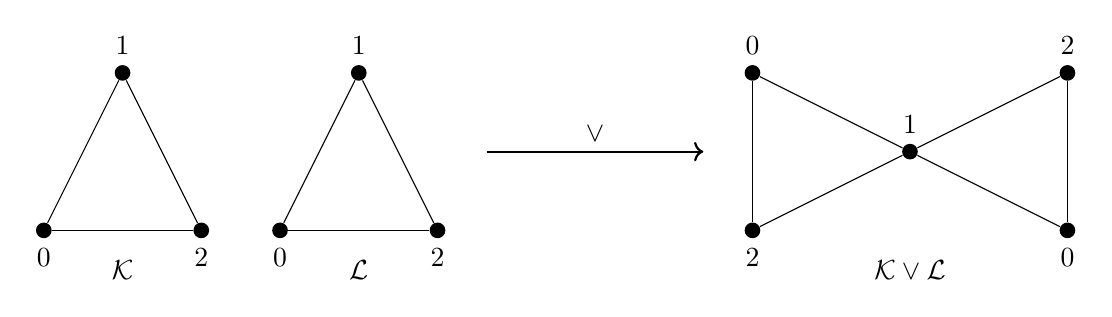
\begin{tikzpicture}
\node[fill=black, circle, inner sep=2pt, label=below:{$0$}] (A) at (0,0) {};
\node[fill=black, circle, inner sep=2pt, label=below:{$2$}] (B) at (2,0) {};
\node[fill=black, circle, inner sep=2pt, label=above:{$1$}] (C) at (1,2) {};
\node[align=center] at (1,-0.5) (label1) {$\mathcal{K}$};

\node[fill=black, circle, inner sep=2pt, label=below:{$0$}] (D) at (3,0) {};
\node[fill=black, circle, inner sep=2pt, label=below:{$2$}] (E) at (5,0) {};
\node[fill=black, circle, inner sep=2pt, label=above:{$1$}] (F) at (4,2) {};
\node[align=center] at (4,-0.5) (label2) {$\mathcal{L}$};

\node[fill=black, circle, inner sep=2pt, label=above:{$0$}] (G) at (9,2) {};
\node[fill=black, circle, inner sep=2pt, label=below:{$2$}] (H) at (9,0) {};
\node[fill=black, circle, inner sep=2pt, label=above:{$1$}] (I) at (11,1) {};
\node[fill=black, circle, inner sep=2pt, label=above:{$2$}] (J) at (13,2) {};
\node[fill=black, circle, inner sep=2pt, label=below:{$0$}] (K) at (13,0) {};
\node[align=center] at (11,-0.5) (label3) {$\mathcal{K} \lor \mathcal{L}$};

\node at (5.5, 1) (AS) {};
\node at (8.5, 1) (AE) {};

\draw (A) -- (B);
\draw (B) -- (C);
\draw (C) -- (A);

\draw (D) -- (E);
\draw (D) -- (F);
\draw (E) -- (F);

\draw (G) -- (I);
\draw (G) -- (H);
\draw (H) -- (I);
\draw (J) -- (K);
\draw (J) -- (I);
\draw (K) -- (I);

\draw [->, thick] (AS) -- node[above] {$\lor$} (AE);
    \end{tikzpicture} 
    \caption{Examples of the wedge of simplicial complexes.}\label{fig:simwejo}
\end{figure}

\begin{lemma}\label{lem:seqhom}
  Let $\mathcal{K}$ be a simplicial complex and let $(L_i)_{i\in [p]}$ be a sequence of subcomplexes of $\mathcal{K}$ for $p \in \N$. If $L_i$ is empty or contractible for each $i \in [p]$ then \[\lVert {\rm Cone}(\mathcal{K}, (L_i)_{i\in [p]}) \rVert \simeq \lVert \mathcal{K} \rVert.\]
\end{lemma}

\begin{proof}
  We know that each ${\rm Cone}(L_i)$ for $i \in [p]$ is contratible. So there is a homotopy equivalence to a one point space. Choose a point in $\lVert \mathcal{K} \rVert$ to which ${\rm Cone}(L_i)$ is contracted to for each $L_i$. The we start with $i = 1$ and can define a homotopy equivalence that keeps $\mathcal{K}$ fixed and contracts the cone over $L_i$ to the chosen point in $\mathcal{K}$. This shows that $\lVert \mathcal{K} \cup {\rm Cone}(L_0) \rVert \simeq \lVert \mathcal{K} \rVert$. The statement follows by induction on $i$. 
\end{proof}

Now consider the complexes $\mathcal{K} = \PowS_{\leq 1}(\{0, 1\})$ and $\mathcal{L} = \PowS_{\leq 1}(\{2, 3\})$. The geometric realization of the join $\mathcal{K} \star \mathcal{L}$ of these complexes can be seen in Figure \ref{fig:simjo}. From the figure it becomese apperent that $\lVert \mathcal{K} \star \mathcal{L} \rVert$ is homeomorphic to $\mathbb{S}^1$.

  \begin{figure}[h!]
  \centering
  \begin{tikzpicture}
\node[fill=black, circle, inner sep=2pt, label=below:{$0$}] (D) at (1,0) {};
\node[fill=black, circle, inner sep=2pt, label=below:{$1$}] (E) at (2,0) {};
\node[align=center] at (1.5,-1) (label3) {$\mathcal{K}$};

\node[fill=black, circle, inner sep=2pt, label=below:{$2$}] (D) at (2,2) {};
\node[fill=black, circle, inner sep=2pt, label=below:{$3$}] (E) at (3,2) {};
\node[align=center] at (2.5,1) (label3) {$\mathcal{L}$};

\node[fill=black, circle, inner sep=2pt, label=above:{$0$}] (G) at (7,2) {};
\node[fill=black, circle, inner sep=2pt, label=below:{$3$}] (H) at (7,0) {};
\node[fill=black, circle, inner sep=2pt, label=above:{$2$}] (I) at (9,2) {};
\node[fill=black, circle, inner sep=2pt, label=below:{$1$}] (K) at (9,0) {};
\node[align=center] at (8,-0.5) (label3) {$\mathcal{K} \star \mathcal{L}$};

\node at (4, 1) (AS) {};
\node at (6, 1) (AE) {};

\draw (G) -- (H);
\draw (H) -- (K);
\draw (K) -- (I);
\draw (I) -- (G);

\draw [->, thick] (AS) -- node[above] {$\star$} (AE);
  \end{tikzpicture}
  \caption{Example of the join of simplicial complexes.}\label{fig:simjo}
  \end{figure}
\end{ex}

The fact that the join of a two points with two points results in a simplicial complex that has a geometric realization that is homeomorphic does not only work with $\mathbb{S}^1$. This fact holds more generally for the n-fold join of 2-point simplicial complexes. 

\begin{lemma}\label{lem:simexkn}
  Let $\mathcal{K}_n := \PowS_{\leq 1}(\{(-1, n), (1, n)\})$ for $n \in \N^+$, then
  \begin{equation*}
    \left\lVert \bigstar_{i=1}^k \mathcal{K}_i \right\rVert \: \cong \: \mathbb{S}^{k-1}.
  \end{equation*}
\end{lemma}

\begin{proof}
  A geometric realization of this complex is as follows
  \begin{equation*}
    f\colon V(\bigstar_{i=1}^k \mathcal{K}_i) \to \R^n, \: (x, i) \mapsto x \cdot e_i
  \end{equation*}
  which means that the vertecies get mapped to the canonical basis vectors of $\R^n$ and their negations. 
  This geometric realization forms the boundary of the $n$-crosspolytope\footnote{This $n$-crosspolytope is $\{(x_1, \ldots, x_n) \in \R^n\colon |x_1| + \cdots + |x_n| \leq 1 \}$. The boundary $\partial P^n$ of the polytope is formed by all points with $1$-norm equal to $1$.} for each $n \in \N^+$. It is homeomorphic to the sphere by the homeomorphism
  \begin{equation*}
    \varphi\colon \mathbb{S}^n \to \partial P^n, \: x \mapsto \lVert x \rVert_1^{-1} \cdot x. 
  \end{equation*}
\end{proof}

\begin{figure}[ht!]
  \centering
  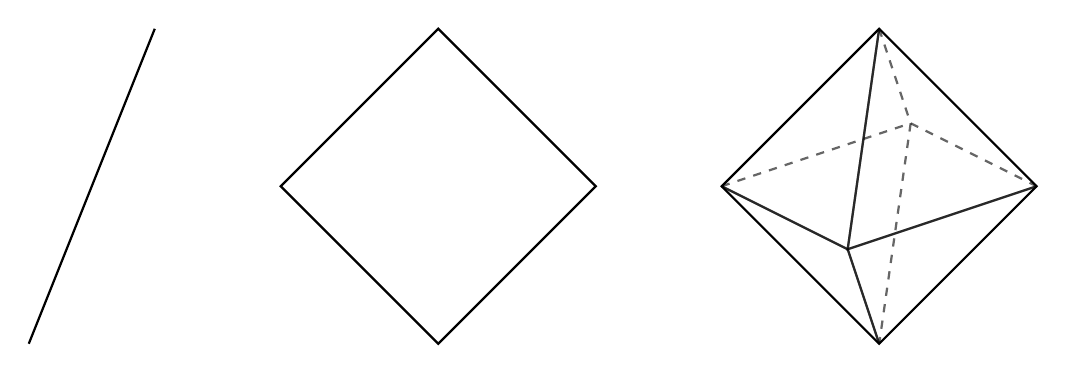
\begin{tikzpicture}[thick,scale=4]

\coordinate (D1) at (-1.8, 0.5);
\coordinate (D2) at (-2.2,-0.5);

\draw (D1) -- (D2);

\coordinate (C1) at (-1.4,0);
\coordinate (C2) at (-0.9,0.5);
\coordinate (C3) at (-0.9,-0.5);
\coordinate (C4) at (-0.4,0);

\draw (C1) -- (C2) -- (C4) -- (C3) -- cycle;

\coordinate (A1) at (0,0);
\coordinate (A2) at (0.6,0.2);
\coordinate (A3) at (1,0);
\coordinate (A4) at (0.4,-0.2);
\coordinate (B1) at (0.5,0.5);
\coordinate (B2) at (0.5,-0.5);

\begin{scope}[thick,dashed,,opacity=0.6]
\draw (A1) -- (A2) -- (A3);
\draw (B1) -- (A2) -- (B2);
\end{scope}
\draw[opacity=0.6] (A1) -- (A4) -- (B1);
\draw[opacity=0.6] (A1) -- (A4) -- (B2);
\draw[opacity=0.6] (A3) -- (A4) -- (B1);
\draw[opacity=0.6] (A3) -- (A4) -- (B2);
\draw (B1) -- (A1) -- (B2) -- (A3) --cycle;
\end{tikzpicture}
  \caption{Cross polytopes in dimensions one, two and three.}
  \label{fig:cross}
\end{figure}

\subsection{Homology Theory}
Now a very important tool in algebraic topology is introduced, namely \textbf{Homology Theory} of topological spaces. For the basic definitions from Category theory and Homological Algebra needed in the following see \cite{rotmann2009}.  

\begin{cons}
  Let $S$ be a finite set and $p \in \mathbb{P}$. Define \[A(S) := \{f \in \Z^S\colon |\im f| < \infty \}\] be maps from $S$ to $Z_p$ with finite image. $A(S)$ is an abelian group together with the operation of pointwise addition of maps.
  Then the set \[\{\mathds{1}_x\colon x\in S\} \subseteq A(S)\] forms a basis of the abelian group $A(S)$.
  Let $T$ be another set. For a map $\varphi\colon S \to T$ define the map $A(T; p)$ as
  \begin{equation*}
    A(\varphi)\colon A(S) \to A(T),\; f \mapsto \sum\limits_{x \in S}f(x)\cdot \mathds{1}_{\varphi(x)}.
  \end{equation*}
  This map is a homomorphisms of abelian groups.
\end{cons}

\begin{proof} 
  The fact that $A(S)$ is abelian follows from the fact that the group $\Z$ is abelian and thus the pointwise addition is associative and commutative, the neutral element is the constant $0$ function and the inverse of an element $f \in A(S)$ is defined as $f^{-1}(s) = -f(s)$ for $s \in S$.

  Now let $f \in A(S)$ and consider the function \[\tilde{f}\colon S \to \Z, \: s \mapsto \sum\limits_{x\in S} \alpha_x \mathds{1}_x(s)\] with $\alpha_x = f(x)$ for all $x \in S$. Let $s \in S$. It follows that
  \begin{equation*}
    \tilde{f}(s) = \sum\limits_{x \in S} \alpha_x \mathds{1}_x(s) = \alpha_s = f(s).
  \end{equation*}

  Now let $f,g \in A(S)$.
  \begin{align*}
    A(\varphi)(f+g^{-1}) &= \sum\limits_{x\in S} (f+g^{-1})(x)\cdot \mathds{1}_{\varphi(x)} \\
                        &= \sum\limits_{x\in S} (f(x)-g(x)))\cdot \mathds{1}_{\varphi(x)} \\
                        &= \sum\limits_{x\in S} f(x)\cdot\mathds{1}_{\varphi(x)} + (-g(x))\cdot \mathds{1}_{\varphi(x)} \\
                        &= \sum\limits_{x\in S} f(x)\cdot\mathds{1}_{\varphi(x)} + \sum\limits_{x\in S} (-g(x))\cdot \mathds{1}_{\varphi(x)} \\
                        &= A(\varphi)(f) + A(\varphi)(g)^{-1}.  
  \end{align*}
\end{proof}

Since the collection of indicator functions is a basis of $A(S)$ it is a convention to write elements of $A(S)$ as formal linear combinations of elements of the generating set $S$. This means the group $A(S)$ can also be represented as
\begin{equation*}
  A(S) = \left\{\sum\limits_{i=1}^k r_i x_i\colon k\in \N, \: \forall i \in \{1, \ldots, k\}\colon x_i \in S, r_i \in \Z\right\}.
\end{equation*}

\begin{thm}\label{thm:isoab}
  Let $S$ be a set and let $B$ be an abelian group. Then \[\Phi\colon \underline{\rm Ab}(A(S), B) \to B^X, \: \varphi \mapsto\varphi \circ \mathds\iota^S\footnote{$\iota^S\colon S \to A(S), \: s \mapsto \mathds{1}_s$}\] is a bijection.
\end{thm}

\begin{proof}
  The map $\Phi$ is a homomorphism in of abelian groups. To this end let $\varphi, \psi \in \underline{\rm Ab}$.
  The claim follows from the fact that $\varphi$ and $\psi$ are homomorphisms and \[(\varphi + \psi)(\mathds{1}_x) = \varphi(\mathds{1}_x) + \psi(\mathds{1}_x).\]
  Let $\varphi \in \underline{\rm Ab}(A(S), B)$ and assume that $\varphi \circ \iota^S = 0$. Then it holds that
  \begin{align*}
    \varphi(f) &= \varphi\left(\sum\limits_{x \in S}f(x) \cdot \mathds{1}_s\right) \\
    &= \sum\limits_{x \in S} f(x) \cdot \varphi(\mathds{1}_s) \\
    &= \sum\limits_{x \in S} f(x) \cdot 0 = 0
  \end{align*}
  for all $f \in A(S)$ and thus $\varphi = 0$. This means $\ker \Phi = \{0\}$.
  Now let $\psi \in B^S$. Then the map \[\xi\colon A(S) \to B, f \mapsto \sum\limits_{x \in S} f(x) \psi(x) \] is a homomorphism by
  \begin{align*}
    \xi(f + g) &= \xi\left(\sum\limits_{x \in S} (f+g)(x) \mathds{1}_x\right) \\
    &= \sum\limits_{x \in S}(f+g)\psi(x) \\
    &= \sum\limits_{x \in S} f(x)\psi(x) + \sum\limits_{x \in S}g(x)\psi(x) = \xi(f) + \xi(g).
  \end{align*}
  And now it follows that $\Phi(\xi) = (\xi \circ \iota^S)(x) = \mathds{1}_x(x) \cdot \psi(x) = \psi(x)$ for all $x \in X$ and hence $\Phi(\xi) = \psi$.
\end{proof}

The Theorem now tells us that any function from $X$ to an abelian group $B$ can be extended into a function from $A(X)$ to $B$ in a unique way. This may become clear looking at the commutative diagram in Figure \ref{fig:com1}.

\begin{figure}[h!]
  \centering
  % https://tikzcd.yichuanshen.de/#N4Igdg9gJgpgziAXAbVABwnAlgFyxMJZABgBpiBdUkANwEMAbAVxiRAA0QBfU9TXfIRQBGUsKq1GLNgCFuvEBmx4CRMuOr1mrRCACCACnYBKbhJhQA5vCKgAZgCcIAWyRkQOCEgBM1HHSwGNgALCAgAaxBqBiwwHRA4CBioKJBgmDoUxDAmBgZougAjGAYABX4VIRAHLEtgnFStaV0AHRb8fwA9Tmo4YKw7BsRiHnsnV2G-L0RRSW02NvoHNH75MZcfKaRZmLi2KAgcHAtUhiKS8uVBNhq6hs0peLaYAA8sOBw4AEI24LocYCLOjLfpcMxcIA
  \begin{tikzcd}
    X \arrow[d, "\iota^X"', hook] \arrow[rd, "\varphi"] &   \\
    A(X) \arrow[r, "\exists!\hat{\varphi}"', dashed]    & B
  \end{tikzcd}
  \caption{Commutative diagram showing the statement of Theorem \ref{thm:isoab}}\label{fig:com1}
\end{figure}

\begin{defin}
  Let $n\in\N$. The \textbf{geometric n-simplex} $\Delta_n$ is defined as
  \begin{equation*}
    \Delta_n := {\rm co}\{e_0\, \ldots, e_n\} \subseteq \R^{n+1}
  \end{equation*}
  where $e_i$ is the $i$-th canonical basis vector of $R_n$ for $i = 0,\ldots,n$. For all $i = 0, \ldots, n$ define the $i$-th face map as
  \begin{equation*}
    d_i\colon \Delta_{n-1} \to \Delta_n,\: (t_0,\ldots,t_{n-1}) \mapsto (t_0, \ldots, t_{i-1}, 0, t_i, \ldots, t_{n-1}).
  \end{equation*}
  Notice that $\im d_i \subseteq \Delta_n$. $\im d_i$ is called the $i$-th face of $\Delta_n$.
\end{defin}

\begin{defin}
  Let $X$ be a topological space and let $n\in \N$ and $p \in \mathbb{P}$. A \textbf{singular $n$-simplex} in $X$ is a continuous map $\sigma \in C(\Delta_n, X)$.
  Now the \textbf{singular $n$-chain group} of $X$ is defined as $C_n(X) := A(C(\Delta_n, X); p)$. An element $\sigma \in C_n(X)$ is called a singular $n$-chain in $X$.
  The map \[\partial_n\colon C_n(X) \to C_{n-1}(X),\: \sigma \mapsto \sum\limits_{i=0}^n(-1)^i(\sigma \circ d_i)\] is called the $n$-th boundary map for $n\in\N^+$. It is a homomorphisms of abelian groups. For $n < 1$ define $\partial_n$ as the zero map as well as all $C_n$ as trivial abelian groups.

  If $Y$ is another topological space and $f \in C(X, Y)$ then $C_n(f)\colon C_n(X) \to C_n(Y)$ defined on the generators $\sigma \in C_n(X)$ as
  \begin{equation*}
    C(f)(\sigma) = f \circ \sigma.
  \end{equation*}
  This map is a homomorphism of abelian groups.
\end{defin}

\begin{lemma}
  The composition $\partial_n \circ \partial_{n+1} = 0$ for all $n \in \N$.
\end{lemma}

\begin{proof}
  See \cite[Theorem 29.1]{MunAlTop}.
\end{proof}

The lemma above is the so called fundamental theorem of homology theory. It allows for the following definition.

\begin{defin}
  Let $X$ be a topological space, then \[C_\bullet(X) := ((C_n(X))_{n\in \Z}), (\partial_n)_{n\in \Z})\] with
  \[C_n(X) = \{0\}, \: \partial_n := 0\] for $n \in \Z\setminus\N$ is a chain complex.
\end{defin}

\begin{lemma}
  Let $X, Y$ be topological spaces and $f \in C(X, Y)$, then \[\forall n\in \N\colon \partial_n \circ C_n(f) = C_{n-1}(f) \circ \partial_n.\]
\end{lemma}

\begin{proof}
  Let $n \in \N^+$ and let $\sigma \in C(\Delta_n, X)$ then
  \begin{align*}
    \partial_n(C_n(f)(\sigma)) &= \partial_n(f\circ\sigma) \\
    &= \sum\limits_{i=0}^n(-1)^if\circ\sigma\circ d_i \\
    &= \sum\limits_{i=0}^n(-1)^iC_{n-1}(f)(\sigma\circ d_i) \\
    &= C_{n-1}(f)(\sum\limits_{i=0}^n(-1)^i(\sigma\circ d_i)) \\
    & = C_{n-1}(f)(\partial_n(\sigma)).
  \end{align*}
\end{proof}

From the previous lemma it is clear that $C_\bullet(f) := (C_n(f))_{n\in \Z}$ with $C_n(f) = 0$ for $n < 0$ is a homomorphism between chain complexes $C_\bullet(X)$ and $C_\bullet(Y)$.

\begin{lemma}\label{lem:cfunc}
  $C_\bullet\colon \underline{\rm Top} \to \underline{\rm C}(\underline{\rm Ab})$ is a functor.
\end{lemma}

\begin{proof}
  Let $X$ be a topological space and let $n \in \N$, then \[C_n(\id_X)(\sigma) = \id_X\circ \sigma = \sigma = \id_{C_n(X)}(\sigma)\]
  for all $\sigma \in C(\Delta_n, X)$ and hence $C_n(\id_X) = \id_{C_n(X)}$.
  For $n < 0$ this is trivial.

  Let $Y, Z$ be topological spaces and $f \in C(X, Y), g\in C(Y, Z)$, then for $n\in \N$ it follows that \[C_n(g\circ f)(\sigma) = g\circ f \circ \sigma = C_n(g)(f\circ \sigma) = (C_n(g) \circ C_n(f))(\sigma)\] for all $\sigma \in C(\Delta_n, X)$ and thus $C_n(g \circ f) = C_n(g) \circ C_n(f)$.
  Again the case for $n < 0$ is trivial.
\end{proof}

\begin{thm}\label{thm:hfunc}
  Let $n \in \N$. Then \[H_n\colon \underline{\rm Top} \to \underline{\rm Ab} \]
  defined by \[H_n(X) := H_n(C_\bullet(X)), \: H_n(f) := H_n(C_\bullet(f))\]
  for a topological spaces $X$ and $Y$ and $f \in \underline{\rm Top}$ is called the $n$-th singular homology group and  is a functor. 
\end{thm}

\begin{proof}
  Follows from the fact that the composition of functors is again a functor and Lemma \ref{lem:cfunc}.
\end{proof}

\begin{thm}\label{thm:hhom}
  Let $X$ and $Y$ be topological spaces. Then if $f, g\in C(X, Y)$ are homotopic maps it follows that \[H_n(f) = H_n(g)\] for all $n \in \N$.
\end{thm}

\begin{proof}
  See \cite[p. 112f]{hatcher}.
\end{proof}

\begin{col}
  Let $X$ and $Y$ be topological spaces and $f \in C(X, Y)$ is a homotopy equivalence between them, then $H_n(f)\colon H_n(X) \to H_n(Y)$ is an isomorphism for all $n \in \Z$.
\end{col}

\begin{proof}
  This follows directly from Theorem \ref{thm:hhom}.
\end{proof}

\begin{ex}
  Take a topological space $X$. Then $H_0(X) \cong \Z^n$ where $n \in \N$ is the number of path-connected components in $X$. 
\end{ex}

The example above implies that the $0$-th homology group of for example a one point space is $\Z$. This complicates some other results in homology theory. Therefore there is a version of the homology groups called \textbf{reduced} homology groups $\tilde{H_n}$ where $\tilde{H}_n(X) = H_n(X)$ for all $n \in\N^+$ and $\tilde{H}_n \oplus \mathbb{Z} = H_n(\Z)$. This means that the $0$-th reduced homology group of a one point space the trivial group is instead of $\mathbb{Z}$.
A detailed derivation of the reduced groups can be found in \cite[p. 110]{hatcher}.

\begin{defin}
  Let $G_\alpha$ be an abelian group for each $\alpha$ in an arbitrary index set $I$. Then the \textbf{external direct sum} of the groups is defined as
  \begin{equation*}
    \bigoplus\limits_{\alpha \in I}G_\alpha = \{(g_\alpha)_{\alpha\in I}\colon g_i\in G_i \: \land \: g_i \neq e_{G_i} \text{ for only finitely many indicies } i \in I\}.
  \end{equation*}
  This is again an abelian group with the operation \[(g)_{\alpha \in I} \cdot (h)_{\alpha\in I} = (g_\alpha \cdot_{G_\alpha} h_\alpha)_{\alpha \in I}.\]
  If $f_\alpha$ is a homomorphism with \[f_\alpha\colon G_\alpha \to H\]  for each $\alpha \in I$ where $H$ is an abelian group. Then
  \begin{equation*}
    \bigoplus\limits_{\alpha\in I}f_\alpha\colon \bigoplus_{\alpha \in I} G_\alpha\to H,\: (g)_{\alpha \in I} \mapsto \sum\limits_{\alpha \in I}f_\alpha(g_\alpha)
  \end{equation*}
  is a well-defined homomorphism since only finitely many summands are non-trivial.
\end{defin}

\begin{defin}
  Let $X$ be a topolgical space and let $A \subseteq X$ be a non-empty closed subspace, that is a deformation retract of a neighborhood in $X$. Then $(X, A)$ is a \textbf{good pair}.
\end{defin}

\begin{lemma}\label{lem:holwe}
  Let $X_\alpha$ be a sequence of topological spaces with basepoints $x_\alpha\in X_\alpha$ and let $\iota_\alpha\colon X_\alpha \to \bigvee\limits_{\alpha \in I}X_\alpha$ for $\alpha \in I$ where $I$ is an arbitrary index set such that $(X_\alpha, x_\alpha)$ are good. Then it holds that the maps $\iota_\alpha$ induce an isomorphism
  \begin{equation*}
    \bigoplus_{\alpha \in I}H_n(\iota_\alpha) \colon \bigoplus\limits_{\alpha\in I} \tilde{H}_n(X_\alpha)\to \tilde{H}_n\left(\bigvee\limits_{\alpha\in I} X_\alpha\right).
  \end{equation*}
\end{lemma}

\begin{proof}
  See \cite[Corollary 2.25]{hatcher}.
\end{proof}

Proofs in the later sections will only involve reasoning about homology groups. Their is a dualized concept of homology called cohomology.
The dualization in the sense of category theory works be replacing the homology groups in the chain complex by $\underline{\rm Grp}(H_n(X); G)$ where $G \in \underline{\rm Ab}$ is an abelian group. There is no need to also develop the theory of cohomology in this thesis nor a need to use it later in the proofs because of the following result. Its called \textbf{Alexander duality} and connects homology and cohomology groups.

\begin{thm}\label{thm:alex}
  Let $n \in \N$. If $A \subseteq \mathbb{S}^n$ is a compact and non-empty subspace and ($\mathbb{S}^n, A$) is triangulable\footnote{This means that $A \subseteq \mathbb{S}^n$ and that there exists a triangulation $\mathcal{K}$ of $\mathbb{S}^n$ and a subcomplex $\mathcal{K}_0 \subseteq \mathcal{K}$ with an homeomorphism $(\mathcal{K}, \mathcal{K}_0) \to (\mathbb{S}^n, A)$.} then
  \begin{equation*}
    \tilde{H}^k(A) \cong \tilde{H}_{n-k-1}(\mathbb{S}^n \setminus A)
  \end{equation*}
  for all $k \in \N$.
\end{thm}

\begin{proof}
  See \cite[Theorem 71.1]{MunAlTop}.
\end{proof}

\begin{defin}
  Let $(G_n)_{n\in\N}$ be a sequence of abelian groups and let $(\varphi_n)_{n\in\N}$ be a sequence of homomorphisms such that
  \begin{equation*}
    \varphi_n\colon G_n \to G_{n-1}
  \end{equation*}
  for $n \in \N^+$ and $\varphi_0\colon G_0 \to 0$.
  The sequence is called \textbf{exact} if
  \begin{equation*}
    \im\varphi_{n+1} = \ker\varphi_n.
  \end{equation*}
  for all $n \in \N$.
  An exact sequence of the form
  \begin{equation*}
    0 \to A \to B \to C \to 0
  \end{equation*}
  that is exact is called a \textbf{short exact sequence}.
\end{defin}

A second important tool linking homology and cohomology groups is the \textbf{universal coefficient theorem}. The next theorem is a version of it.

\begin{thm}\label{thm:uct}
Let $C_n(X)$ be a chain complex of free abelian groups and the corresponding homology groups $H_n(X)$ of $C_n(X)$ for a topological space $X$, then the cohomology groups $H^n(X; G)$ for a abelian group $G$ are determined by the exact sequence
  \begin{equation*}
    0 \to {\rm Ext}(H_{n-1}(X), G) \to H^n(X; G) \to \underline{\rm Ab}(H_n(X), G) \to 0.
  \end{equation*}
  For the definition of the ${\rm Ext}$-functor look in \cite[p. 195]{hatcher}.
\end{thm}

\begin{proof}
  See \cite[Chapter 3.1]{hatcher}.
\end{proof}

We will need only the following corollary from this theorem.

\begin{col}\label{col:hntriv}
  Let $C_n(X)$ be a chain complex of free abelian groups and $H_n(X)$ the corresponding homology groups with $H_n(X) \cong 0$ for $0 \leq n \leq k \in \N$. Then the cohomology groups are all trivial up to $k$. 
\end{col}

\subsection{Theorem of Mayer-Vietoris}
Often we can calculate the homology of simple subspaces of a larger space and want to deduce the homology of the larger space from them.
This can be accomplished with the \textbf{Mayer-Vietoris-Sequence} which is a homological version of the \textbf{Van Kampen-Theorem} (see \cite[Chapter 1.2]{hatcher}).

\begin{thm}\label{thm:mvs}
  Let $X$ be a topological space and let $A, B \subseteq X$ subspaces of $X$ such that \[X = \dot{A} \cup \dot{B}, \: A \cap B \neq \emptyset.\]
  The \textbf{Mayer-Vietoris-Sequence}
  \begin{equation*}
    \ldots \to H_n(A\cap B) \overset{\Phi}{\to} H_n(A) \oplus H_n(B) \overset{\Psi}{\to} H_n(A \cup B) \overset{\partial}{\to} H_{n-1}(A\cap B) \to \ldots \to 0
  \end{equation*}
  is an exact sequence where the mappings $\Phi$ and $\Psi$ are defined as
  \begin{align*}
    &\Phi\colon H_n(A\cap B) \to H_n(A) \oplus H_n(B),\: z + B_n(A\cap B) \mapsto (z+B_n(A), -z + B_n(B)), \\
    &\Psi\colon H_n(A) \oplus H_n(B) \to H_n(A\cup B), \: (z_1+ B_n(A), z_2 + B_n(B)) \mapsto (z_1 + z_2) + B_n(A \cup B).
  \end{align*}
\end{thm}

\begin{proof}
  For a detailed derivation of this Theorem look at \cite[p. 149]{hatcher}. 
\end{proof}

\begin{ex}
  The homology group of the $n$-dimensional sphere $\mathbb{S}^n$ are as follows
  \begin{equation*}
    H_k(\mathbb{S}^n) \cong \begin{cases}
      0, &n \neq k, \\
      \mathbb{Z}, &n = k,
    \end{cases}
  \end{equation*}
  for $k \in \Z$.
\end{ex}

\begin{proof}
  Let $A$ be the upper hemisphere and $B$ the lower hemisphere of $\mathbb{S}^n$. Then $A\cap B = \mathbb{S}^{n-1}$. Consider the Mayer-Vietoris sequence of this decomposition
  \begin{equation*}
    \ldots \overset{\partial'}{\to} H_k(\mathbb{S}^{n-1}) \to H_k(A) \oplus H_k(B) \to H_k(\mathbb{S}^n) \overset{\partial}{\to} H_{k-1}(\mathbb{S}^{n-1}) \to \ldots \to 0.
  \end{equation*}
  Since $A$ and $B$ are contractible it follows that $H_n(A) \cong H_n(B) \cong 0$ for all $n \in N$. This means that
  \begin{align*}
    0 &= \im \Psi = \ker \partial_k \\
    H_k(\mathbb{S}^{n-1}) &= \ker \Phi = \im \partial_{n+1}.
  \end{align*}
  We get that the maps $\partial\colon H_k(\mathbb{S}^n) \to H_{k-1}(\mathbb{S}^{n-1})$ are isomorphism. And thus with the fact that $H_1(\mathbb{S}^1) \cong \Z$ the claim is proven by induction on $k$.\footnote{The fact that the first homology group of $\mathbb{S}^1$ is isomorphic to $\Z$ can easily be proven with another type of homology, namely simplicial homology \cite[p. 106]{hatcher}. And since the singular and simplicial homology groups are isomorphic for triangulable spaces it can be deduced that $H_1(\mathbb{S}^1) \cong \Z$ also in the singular case. A triangulation of $\mathbb{S}^1$ is the circle graph with three vertecies.}
\end{proof}

\section{$L_0$-Groups, connection between extrem ameanability and chromatic numbers}
%TODO: cite paper of friedrich martin with the definitions of raikov and submeasures
In this chapter, we want to establish a connection between the extrem ameanability of a $L_0$-Group and the boundedness of the chromatic numbers of a sequence of graphs.
These graphs will be constructed using the structure of the $L_0$-groups.

\begin{defin}
  Let $\mathcal{A}$ be a boolean algebra and $\mu\colon \mathcal{B} \to [0, \infty)$. The map $\mu$ is called a \textbf{submeasure} if
  \begin{enumerate}
    \item $\mu(0) = 0$,
    \item $\forall A, B \in \mathcal{A}\colon A \leq B \Rightarrow \mu(A) \leq \mu(B)$,
    \item $\forall A, B \in \mathcal{A}\colon \mu(A \lor B) \leq \mu(A) + \mu(B)$.
  \end{enumerate}
\end{defin}

From here a submeasure on a set $X$ is a submeasure on the power set algebra on $X$.

\begin{defin}
  Let $X$ be a set. Then ${\rm PartFin}(X)$ is the set of all finite partitions of $X$, which means:
  \begin{equation*}
    {\rm PartFin}(X) := \left\{ \mathcal{A} \subseteq \P(X)\colon (\forall A,B \in \mathcal{A}\colon A \cap B = \emptyset) \: \land \: \bigcup\mathcal{A} = X \: \land \: \left| \mathcal{A} \right| < \infty \right\}.
  \end{equation*}
  Let $\P_1, \P_2 \in {\rm PartFin}(X)$. $\P_1$ is said to \textbf{refine} $\P_2$ ($\P_2 \preccurlyeq \P_1$) if
  \begin{equation*}
    \forall A \in \P_1\exists B \in \P_2\colon A \subseteq B.
  \end{equation*}
  For every $\P \in {\rm PartFin}(X)$ define the map $\iota_\P\colon X \to \P$ with
  \begin{equation*}
    \iota_\P\colon x \mapsto \begin{cases}
      &A_1, \: \text{if } x \in A_1, \\
      &A_2, \: \text{if } x \in A_2, \\
      &\vdots \\
      &A_n, \: \text{if } x \in A_n,
    \end{cases}
  \end{equation*}
  where $k = \left|\P\right|$.    
  %TODO: is this needed?
  The set ${\rm PartFin}_\mu(X)$ contains all finite partitions of $X$ but with the additional constraint that they have to be measurable with respect to a submeasure $\mu$ on the boolean algebra of subsets of $X$. 
\end{defin}

%TODO: directed set in appendix? or definition above?
\begin{thm}\label{thm:algdirected}
  Let $X$ be a set. Then the set ${\rm PartFin}(X)$ together with the binary operation $\preccurlyeq$ is a directed set.
\end{thm}

% TODO: picture of refinments of the square
\begin{proof}
  Reflexivity and transitivity follow directly from the reflexivity and transitivity of the $\subseteq$ relation.
  Now let $\P_1, \P_2 \in {\rm PartFin}(X)$. Define $\P_3 := \{ P \cap P' \colon P \in \P_1, \:P' \in \P_2 \}$.
  Since for any two sets $A, B$ it holds that $A \cap B \subseteq A$ and $A \cap B \subseteq B$ it follows that
  \begin{equation*}
    \P_1 \preccurlyeq \P_3 \land \P_2 \preccurlyeq \P_3.
  \end{equation*}
\end{proof}

\begin{rem}\label{rem:partfinsze}
  If $X$ is an infinite set then ${\rm PartFin}(X)$ is also infinite.
\end{rem}

\begin{proof}
  Define $\P \subseteq {\rm PartFin}(X)$ as follows
  \begin{equation*}
    \P := \Big\{ \{ \{x\}, \: X\setminus\{x\}\}\colon \: \forall x \in X \Big\}.
  \end{equation*}
  It is now clear that $\left| \P \right| = \left| X \right|$ and since $\P \subseteq {\rm PartFin}(X)$ it follows that 
  \begin{equation*}
    \left| X \right| \leq \left| {\rm PartFin}(X) \right|.
  \end{equation*}
\end{proof}

\begin{defin}
  Let $X$ and $Y$ be sets. A step function $f\colon X \to Y$ with finite range induces a finite partion on X called $\P_f$ in the following way
  \begin{equation*}
    \P_f := \{f^{-1}(\{y\})\colon \forall y \in Y\}.
  \end{equation*}
  This is a well-defined finite partion because of the assumption that $f$ has finite range.
\end{defin}

\begin{defin}
  Let $(X, \mathcal{B})$ be a measureable space and let $\mu\colon \mathcal{B} \to [0, \infty]$ be a submeasure on $X$. Then the set
  \begin{equation*}
    S(\mu, G) := \left\{ f: X \to G\colon f \:\:\mu-\text{measureable} \: \land \: \left| f(X) \right| < \infty \right\}
  \end{equation*}
  for a group $G$ is the set of all measurable step functions with finite range on $X$ and values on $G$.
\end{defin}

This set of simple functions is dense in the set $L_0(\mu, G)$. But since in general $L_0(\mu, G)$ is not a metric space, the standard metric notion of completion does not work. Instead it is true that the Raikov completion $\widehat{S(\mu, G)} = L_0(\mu, G)$. Look at \cite{} for further information of this completion. This fact about the simple functions is needed because of the following theorem:
\begin{thm}
  
\end{thm}

In the following that symbols $\bar{1}$ represents the constant function which sends each element to 1 in the set $S(\mu, \Z)$. 

\begin{lemma}\label{lem:1}
  Let $(X, \mathcal{B})$ be a measurable space and let $\mu$ be a submeasure on $X$. Additionally, let $\P \in {\rm PartFin}(X)$ and $\varepsilon \in \R_{>0}$ then for $f,g \in \Z^\P$ with $f - g \in \bar{1} + V_\varepsilon$ it follows that $f$ and $g$ are connected in $\Gamma_\varepsilon^\P(\mu)$ by an edge.
\end{lemma}

\begin{proof}
  \begin{align*}
    f - g \in \bar{1} + V_\varepsilon   &\iff \mu(\{x \in X\colon (f-g)(x) \neq 1\}) < \varepsilon \\
                                      &\iff \mu(\{x \in X\colon f(x) \neq g(x) + 1\}) < \varepsilon \\
                                      &\iff \mu(\bigcup \{A \in \P \colon f(A) \neq g(A) + 1\}) < \varepsilon
  \end{align*}
\end{proof}

\begin{lemma}\lemma{lem:colve}
  Let $X$ be an infinite set, $\mu\colon \mathcal{B} \to [0, \infty]$ a submeasure on $X$ where $\mathcal{B}$ is a $\sigma$-algebra and let $G$ be an abelian group. Then the following are equivalent:
  \begin{enumerate}
    \item $L_0(\mu, G)$ is extremely ameanable,
    \item $\forall \varepsilon > 0$ there is no finite bound on $\chi(\Gamma_{\varepsilon}^{\mathcal{P}}(\mu))$, where $\mathcal{P} \in {\rm PartFin}(X)$.
  \end{enumerate}
\end{lemma}

%TODO: define S(\mu, G) and the property of inheritance of ameanability through the raikov completion
%TODO: syndetic set definition
%TODO: correctly cite pestov
\begin{proof}
  Assume there exists a finite bound $d \in \N$ for the chromatic number for some $\varepsilon \in \R_{>0}$, i.e.
  \begin{equation*}
    \forall \P \in {\rm PartFin}(X)\colon \chi(\Gamma_\varepsilon^{\P}(\mu)) \leq d. 
  \end{equation*}
  Given this assumption we claim that the the group $L_0(\mu, \Z)$ is not extremely ameanable. To this end choose a coloring of $\Gamma_{\varepsilon}^{\P}(\mu)$ called $c_{\P}\colon \Z^{\P} \to \{1, \ldots, d\}$ for every $\P \in {\rm PartFin}(X)$. Consider the family of sets
  \begin{equation*}
    \mathcal{A} := \{\{ \P \in {\rm PartFin}(X)\colon \P_0 \preccurlyeq \P\}\colon \P_0 \in {\rm PartFin}(X)\}.
  \end{equation*} 
  This is a well-defined filter basis by Theorem \ref{thm:algdirected} and Lemma \ref{lem:filbas}. From Theorem \ref{thm:ulfil} it follows that there is an ultrafilter $\mathcal{U}$ containing the filter $\mathcal{F}(\mathcal{A})$.
 Let $\P_f$ be the finite partion of $X$ induced by $f \in S(\mu, \Z)$. Define $f_\P \in \Z^\P$ for all finite partitions $\P$ refining the partion $\P_f$ as
  \begin{equation*}
    f_\P(A) = k \iff \exists B \in f^{-1}(\{k\})\colon A \subseteq B. 
  \end{equation*}
  This functions is well-defined because of the definition of refinment of partitions and thus also $f \in S(\mu, \Z)$.
  Now define a coloring $c: S(\mu, G) \to \{1, \ldots, d\}$ of $S(\mu, G)$ as the limit over the ultrafilter
  \begin{equation*}
    c(f) := \lim\limits_{\P \to \mathcal{U}} c_{\P}(f_\P).
  \end{equation*}
  Let $X_i := \{f \in S(\mu, \Z)\colon c(f) = i\}$ for each $i = 1, \ldots, d$ which is a cover of $S(\mu, \Z)$ and let $f, g \in \Z^\P$. By Lemma \ref{lem:1} it follows that $c_\P(f) \neq c_\P(g)$ for $f - g \in \bar{1} + V_\varepsilon$.
  In the limit of the ultrafilter $\mathcal{U}$ we get $(\bar{1} + V_\varepsilon) \cap (X_i - X_i)$ for each $i = 1, \ldots, d$ and thus $X_i - X_i$ is not dense at $\bar{1}$. By Pestovs characterization \cite[Theorem 3.4.9]{PestovDyn} of extrem amenability it follows that $S(\mu, \Z)$ is not extremely ameanable. Hence, $L_0(\mu, \Z)$ is not extremly ameanable by Theorem \ref{}. 

  For the second implication suppose that $S(\mu, G)$ is not extremely ameanable. Let $d \in \N$ and let $S_1, \ldots, S_d$ be a finite covering of $S(\mu, G)$ such that there is an $i \in \{1, \ldots, d\}$ with $G \neq \overline{S_i - S_i}$. The existence of such an finite covering with an element that is not everywhere dense follows from Pestovs characterization of extreme ameanability \cite[Theorem 3.4.9]{PestovDyn}.
  Now let $S := S_i$ and let $f \in S(\mu, G) \setminus \overline{S - S}$. It follows that there exist $W \in \mathcal{N}_G(e_G)$ and $\varepsilon \in \R_{>0}$ such that
  \begin{equation*}
    (f + W_\varepsilon) \cap (S - S) = \emptyset
  \end{equation*}
  for $W_\varepsilon := \{h \in S(\mu, G)\colon \mu(\{x\in X\colon h(x) \notin W\}) < \varepsilon\}$ since $f$ is not in the closure of $S - S$. 
  Now let $V_\varepsilon := \{h \in S(\mu, G)\colon \mu(\{x\in X\colon h(x) \neq e_G\}) < \varepsilon\}$. Since $e_G \in W$ it follows that $V_\varepsilon \subseteq W_\varepsilon$ and hence
  \begin{equation*}
    (f + V_\varepsilon) \cap (\overline{S - S}) = \emptyset.
  \end{equation*}
  Define the partition $\P_f$ induced by $f$.
  Now let $\P \in {\rm PartFin}(X)$ with $\P_f \preccurlyeq \P$ and let $k \in \Z^\P$.
  Define
  \begin{equation*}
    g_k\colon X \to G, \: g_k(x) \mapsto k(\iota_\P(x))f(x)
  \end{equation*}
  which is an element of $S(\mu, G)$ and define the mapping $c\colon \Z^\P \to \{1,\ldots, d\}$ as
  \begin{equation*}
    c\colon k \mapsto i \iff g_k \in S_i.
  \end{equation*}

  \textbf{Claim:} The mapping $c$ is a coloring of the graph $\Gamma_\varepsilon^\P(\mu)$. To this end suppose there are two nodes $k, l \in \Z^\P$ which are connected and have the same color $i \in \{1, \ldots, d\}$. Let $B := \bigcup\{A\in\P\colon k(A) \neq l(A) + 1\}$. It holds that $\mu(B) \leq \varepsilon$ since $k$ and $l$ are connected in $\Gamma_\varepsilon^\P(\mu)$. For $x \in X\setminus B$ it holds that
  \begin{equation*}
    g_k(x) - g_l(x) = k(\iota_\P(x))f(x) - l(\iota_\P(x))f(x) = (k(\iota_\P(x)) - l(\iota_\P(x)) f(x) = f(x)
  \end{equation*}
  since $k(A) = l(A) + 1$ for $x \notin B$. It follows that
  \begin{equation*}
    \mu(\{x\in X\colon g_k(x) - g_l(x) \neq f(x)\}) < \varepsilon.
  \end{equation*}
  which means $g_k - g_l \in f + V_\varepsilon$. Furthermore we have $g_k, g_l \in S_i$ becasue of the definition of $c$. Hence $g_k - g_k \in (f + V_\varepsilon) \cap (S_i - S_i) \lightning$.
  This proofs the claim that $c$ is a coloring of $\Gamma_\varepsilon^\P(\mu)$ with $d$ colors.
\end{proof}

\section{The Borsuk-Ulam Theorem and a generalization}\label{sec:borsuk}

The following section describes the Borsuk-Ulam theorem and an important generelization by Volovikov needed to prove the following claim:
\begin{thm}\label{thm:confun}
  If $p \in \mathbb{P}$ and $n, l \in \mathbb{N}$ with $n \geq l$ such that
  \begin{equation*}
    d(p-1) \leq l-1,
  \end{equation*}
  then for every continuous map $f\colon\lVert K_p(n,l)\rVert \to \mathbb{R}^d$ there is a point in $\lVert K_p(n,l)\rVert$ whose $\Z_p$-Orbit is mapped to a single point in $\mathbb{R}^d$ by $f$.
\end{thm}
This theorem will be needed later to prove a bound on the chromatic numbers of the graphs $\Gamma(\mu, \P, \varepsilon)$.
An important tool needed in the proof of Theorem \ref{thm:confun} is a result of Volovikov which he described in \cite{vol1980}. It is a generalization of the Borsuk-Ulam theorem.
\begin{lemma}\label{lem:vol}
  Let $X$ be a connected paracompact Hausdorff space, acted on without fixed points by a cyclic group $\Z_p$ of prime order $p$. For any continuous function $f\colon X \to M$ and generator of $T \in \Z_p$ let
  \begin{equation*}
    A(f) := \{x\in X\colon f(x) = f(Tx) = \cdots = f(T^{p-1}x)\}
  \end{equation*}
  be the set of points of which the $\Z_p$-orbit is mapped by $f$ to a single point. Suppose that $\tilde{H}^i(X; \Z_p) = 0$ for $0 < i < n$ and $M$ is a compact $\Z_p$ orientiable topological manifold of dimension $m$. If the map $f^*\colon \tilde{H}^n(X; \Z_p) \to \tilde{H}^n(M; \Z_p)$ has zero image then the cohomological dimension over $\Z_p$ of $A(f)$ is at least $n-m(p-1)$. 
\end{lemma}

In his book ``Using the Borsuk-Ulam Theorem`` \cite{using2003} Matoušek compiled various formulations of the Borsuk-Ulam theorem and described it can be generalized with the concept of $\Z_2$ spaces and more generally whith $E_nG$ spaces, there $G$ is a group. In our case $G = \Z_p$ and instead of two there will be $p \in \mathbb{P}$ points that get mapped to the same point by any continuous function. 

\subsection{The simplicial complex $K_p(n, l)$}

% TODO: illustration of component interval of a function
\begin{defin}
  Let $n, p \in \N$, then $\tau \subseteq [n+1] \times [p]$ is called a \textbf{partial function} if \[\restr{\tau}{\dom(\tau)} = \tau \cap (\dom(\tau) \times [p])\] is a function. Let $\tau_1, \tau_2$ be partial functions from $[n+1]$ to $[p]$. Now define
  \begin{equation*}
    \tau_1 \subseteq_f \tau_2 \longeq \dom(\tau_1) \subseteq \dom(\tau_2) \: \land \: \forall k \in \dom(\tau_1)\colon \tau_1(k) = \tau_2(k).
  \end{equation*}
  A \textbf{component interval} of $\tau$ is any maximal interval $I \subseteq [n+1]$ such that $\tau$ is constant on $I \cap \dom(\tau)$. Define $\mathbb{I}(\tau)$ to be the set of component intervals of $\tau$. 

  In addition to that let $f, g$ be partial functions from the set $X$ to set $Y$ with $\dom(f) \cap \dom(g) = \emptyset$ and define 
  \begin{equation*}
    f \uplus g: \dom(f) \cup \dom(g) \to Y, \: x \mapsto \begin{cases}
      f(x), \: x \in \dom(f), \\
      g(x), \: x \in \dom(g).
    \end{cases}
  \end{equation*}
\end{defin}

\begin{defin}
  Let $l \in \N$ and $p \in \mathbb{P}$. Let $V_p(n, l) = P([n+1], [p])$ with the additional properties
  \begin{enumerate}[label=\roman*.)]
    \item $\forall \tau \in V_p(n,l)\colon n - l \leq |\dom(\tau)|$,
    \item $\forall \tau \in V_p(n,l)\colon \left|\mathbb{I}(\tau)\right| \leq l+1$.
  \end{enumerate}
\end{defin}

\begin{defin}\label{defin:kpnl}
  Let $K_p(n,l)$ be an abstract simplicial complex with
  \begin{enumerate}[label=\roman*.)]
    \item $V(K_p(n,l)) = V_p(n,l)$,
    \item the simplicies in $K_p(n,l)$ are chains of $V_p(n,l)$ with repect to $\subseteq_f$.
  \end{enumerate}
  This complex is a $\Z_p$ complex with the action
  \begin{equation*}
    \Z_p \times V_p(n,l) \to V_p(n,l), \: (k, \tau) \mapsto \lambda(k, \tau) = k +_f \tau,
  \end{equation*}
  with $\dom(k +_f \tau) = \dom(\tau)$ and $\forall i\in \dom(k +_f \tau)\colon (k+_f\tau)(i) = k +_p \tau(i)$.
\end{defin}

\begin{defin}
  Let $n \in \N$ and $p \in \mathbb{P}$. Define $S_p(n)$ as the abstract simplicial complex with
  \begin{enumerate}[label=\roman*.)]
    \item $V(S_p(n)) = \{\tau\colon [n+1]\to [p]\colon |\dom(\tau)| = 1\}$,
    \item $\sigma \in S_p(n)\setminus\emptyset \: \longeq \: \forall \tau_1,\tau_2\in\sigma\colon \: (\tau_1 \neq \tau_2) \Rightarrow (\dom(\tau_1) \cap \dom(\tau_2) = \emptyset)$.
  \end{enumerate}
\end{defin}

\begin{defin}
  Let $n \in \N$ and $p\in\mathbb{P}$. For $a \in (\Z_p\setminus\{0\})^{n+1}$ define $S_p(n,a)$ as
  \begin{equation*}
    S_p(n,a) := \{0, a(0)\} \star \{0,a(1)\} \star \ldots \star \{0,a(n)\}.
  \end{equation*}
\end{defin}

\begin{rem}\label{rem:s}
  By Lemma \ref{lem:simexkn} it holds that $\lVert S_p(n,a) \rVert \cong \mathbb{S}^{n}$ for $n\in\N$.
\end{rem}

Now, our goal is to show that the complex has all trivial reduced cohomology groups $\tilde{H}^i(K_p(n,l); \Z_p)$ with coefficients in $\Z_p$ such that we can apply lemma \ref{lem:vol}. Since $\Z_p$ together with $+_p$ and the multiplication of the natural numbers $\hspace*{-5px}\mod p$ is a field, it is sufficient to show that the reduced homology groups $\tilde{H}_i(K_p(n,l); \Z_p)$ are trivial. The triviality of the cohomology groups follows from the universal coefficient theorem \ref{thm:uct}. 

\begin{lemma}
  Let $n \in \N$ and let $p \in \mathbb{P}$. Then
  \begin{equation*}
    \lVert K_p(n,n) \rVert \: \simeq \: \left\lVert\bigvee_{i=1}^{(p-1)^{n+1}}\hspace*{-10px}\mathbb{S}^{n}\right\rVert.
  \end{equation*}
\end{lemma}

\begin{proof}
  First notice that $\Z_p \cong \bigvee_{i=1}^{p-1}\mathbb{S}^0 =: S$ with basepoint $1$ via the isomorphism
  \begin{equation*}
    V(\Z_p) \to V(S), \: k \mapsto \begin{cases}
      &[(1, 1)]_\sim, \: k = 0, \\
      &[(-1,k)]_\sim, \: k \neq 0.
    \end{cases}
  \end{equation*}
  Furthermore it holds that $\lVert S_p(n) \rVert \simeq \left\lVert \bigvee_{i=0}^n\Z_p \right\rVert \simeq \left\lVert \bigvee_{i=0}^n\bigvee_{j=1}^{p-1}\mathbb{S}^0 \right\rVert$ and thus
  \begin{equation*}
    \lVert S_p(n) \rVert \simeq \left\lVert \bigvee_{a\in(\Z_p \setminus {0})^{n+1}} \hspace*{-17px}S_p(n,a) \right\rVert \overset{\ref{rem:s}}{\simeq} \left\lVert \bigvee_{a\in(\Z_p \setminus {0})^{n+1}}\hspace*{-15px}\mathbb{S}^n \right\rVert.
  \end{equation*}

  It is clear that $V(S_p(n)) \cong V_p(n,n)$ because the vertecies in $\sd(S_p(n))$ are maximal chains in $S_p(n)$ which are the total functions from $[n+1]$ to $[p]$ by definition and thus $K_p(n,n) \cong \sd(S_p(n))$. By Lemma \ref{lem:sdsimeq} it follows that
  \begin{equation*}
    \lVert K_p(n, n) \rVert \simeq \left\lVert \bigvee_{a\in(\Z_p \setminus {0})^{n+1}}\hspace*{-15px}\mathbb{S}^n \right\rVert \simeq \left\lVert \bigvee_{i=1}^{(p-1)^{n+1}}\hspace*{-10px}\mathbb{S}^n \right\rVert
  \end{equation*}
  since $\left|(\Z_p\setminus\{0\})^{n+1}\right| = (p-1)^{n+1}$.
\end{proof}

In the following it will be needed to show that $K_p(n,n)$ has also a wedge-decomposition similiar to $S_p(n)$.
\begin{defin}
  Let $n\in\N$ and $p\in \mathbb{P}$. Define the abstract simplicial complex $K_p(n,a)$ for $a \in (\Z_p\setminus\{0\})^{n+1}$ as
  \begin{equation*}
    K_p(n,a) = \{\tau \in K_p(n,n)\colon \forall k\colon\dom(\tau)\colon \tau(m) = 0 \: \lor \: t(m) = a(m)\}\}.
  \end{equation*}
\end{defin}

\begin{rem}\label{rem:kcongs}
  Let $n,l\in\N$ with $n \geq l$, $p\in\mathbb{P}$ and $a\in (\Z_p\setminus\{0\})^{n+1}$. It holds that
  \begin{align*}
    K_p(n,a) &\cong \sd(S_p(n,a)), \\
    K_p(l,l) &\cong \sd(S_p(l)).
  \end{align*}
\end{rem}

\begin{proof}
  Rememeber that the vertecies of $\sd(S_p(n,a))$ are the total chains in $S_p(n,a)$ which are isomorphic to $V_p(n,n)$ which means they represent total functions which are either 0 or have the same value as the function $a$ which is the definition of an element in $K_p(n,a)$. The same argument can be applied for the second claim $K_p(l,l) \cong \sd(S_p(l))$
\end{proof}

Now the following decomposition of $K_p(n,n)$ can be proven:
\begin{lemma}\label{lem:kpka}
  Let $n\in\N$ and $p\in\mathbb{P}$. Then it follows that
  \begin{equation*}
    \left\lVert K_p(n,n) \right\rVert \simeq \left\lVert \bigvee_{a\in(\Z_p\setminus\{0\})^{n+1}}\hspace*{-24px}K_p(n,a)\right\rVert.
  \end{equation*}
\end{lemma}
\begin{proof}
  Define $D_n$ as a simplicial complex with
  \begin{itemize}
    \item $V(D_n) = P([m], 0)$,
    \item the simplicies are chains with respect to $\subseteq_f$,
  \end{itemize}
  and define $\bar{0}$ as the total, constant zero function. Note that $D_n \subseteq K_p(n,n)$ and that $D_n \subseteq K_p(n,a)$ for all $a \in (\Z_p\setminus \{0\})^{n+1}$ by definition.
  Also note that $\bigvee\limits_{a\in(\Z_p\setminus\{0\})^{n+1}}\hspace*{-24px}K_p(n,a) = K$ contains $(p-1)^{n+1}$ copies of $D_n$ glued together at $\bar{0}$ and $K_p(n,n)$ contains one copy of $D_n$. $D_n$ is contractible since it is the barycentric subdivision of $\{0\}^{*(n+1)}$ which is the $(n+1)$-fold join of the one point space which is the same as taking $(n+1)$ nested cones of this space. Since taking a cone always produces a contractible space this space is contractible and the barycentric subdivision keeps the homotopy type. Now collapse all copies of $D_n$ in $K$ and collapse the one copy in $K_p(n,n)$ to $\bar{0}$. Then the two sets $K_p(n,n)$ and $K$ are isomorphic by sending a $\tau \in V(K_p(n,n))$ to the component of $K$ where $\tau \subseteq_f a$. Since the simplicies  in $K_p(n,n)$ are chains with respect to $\subseteq_f$ this means that if the greatest element of a chain lies in the component $K_p(n,a)$ for some $a$ in $K$ the whole chain is contained in this component meaning the simplicies are maintained by this isomorphism. 
\end{proof}

\begin{defin}
  Define $L_p(n,l)$ as a subcomlex of $K_p(n,n)$ with \[\forall\tau\in V(L_p(n,l))\colon |\mathbb{I}(\tau)| \leq l+1 \]
  and define $J_p(n,l)$ as a subcomplex of $K_p(n,l)$ with \[\forall \tau \in V(J_p(n,l))\colon |\dom(\tau)| \geq n-l.\]
\end{defin}

Now note that $K_p(n,l) = J_p(n,l) \cap L_p(n,l)$. We can used this fact for applying the Mayer-Vietoris-sequence for finding the homology groups of $K_p(n,l)$. This means we have to firstly study the complexes $J_p(n,l)$ and $L_p(n,l)$ and show that their homology groups are trivial up to some point.

We start our analysis with the subcomplex $L_p(n,l)$. Notice that if we compare $K_p(l,l)$ to $L_p(n,l)$ than $L_p(n,l)$ contains additional partial functions namely all the functions with a domain not contained in $[l+1]$. We will show that we can extend the complex $K_p(l,l)$ by adding cones to specific subcomplexs such that we get a new complex that is isomorphic to $L_p(n,l)$. The intuitition behind this idea is that the added cone points and the join of already existing partial functions will act like the missing functions with large domain. 

\begin{defin}
  Let $\mathcal{K}$ be a simplicial complex, $p,m \in \N$ and let $(L_\sigma)_{\sigma \in P([m],[p])}$ be a family of subcomplexes of $\mathcal{K}$ such that $L_\sigma \subseteq L_\tau$ if $\tau \subseteq \sigma$. Define the complex ${\rm Cone}(\mathcal{K}, (L_\sigma)_{\sigma\in P([m],[p])})$ inductively. Firstly let $\mathcal{K}^0 = \mathcal{K}$ and let $L_\sigma^0 = L_\sigma$ for all $\sigma \in P([m],[p])$. Now define $X^k$ and $L_\sigma^k$ by induction on $k \leq m$ for $\sigma \in P([k+1,m], [p])$ as
  \begin{align*}
    \mathcal{K}^{k+1} &= {\rm Cone}(\mathcal{K}^k, (L^k_{(k,i)})_{i\in [p]}), \\
    L^{k+1}_\sigma &= {\rm Cone}(L^k_\sigma, (L^k_{(k,i) \uplus \sigma})_{i\in [p]})
  \end{align*}
  where $(j,i)$ denotes the partial function $\tau\colon [m] \to [p]$ with $\dom(\tau) = \{j\}$ and $\tau(j) = i$. Define ${\rm Cone}(K, (L_\sigma)_{\sigma \in P([m],[p])}) =: \mathcal{K}^m$.
  Addtionally this definition also works for a set $Y \subseteq [m]$ and all $\sigma \in P(Y, [p])$ only looking at partial functions with a resticted domain because $Y$ inherits the natural order of $\N$.
\end{defin}

The well-definition of the induction step follows from the assumption that $A_\sigma \subseteq A_\tau$ if $\tau \subseteq \sigma$.

\begin{lemma}\label{lem:ecsimeq}
  Let $\mathcal{K}$ be a simplicial complex and let $(L_\sigma)_{\sigma \in P(m,p)}$ be a sequence of subcomplexes for $p,m \in \N$ empty or contractible then \[\lVert \mathcal{K} \rVert \simeq \lVert {\rm Cone}(\mathcal{K}, (L_\sigma)_{\sigma \in P(m,p)})\rVert.\]  
\end{lemma}

\begin{proof}
  We prove the claim by induction. So let $k = 0$. Then the claim follows directly from lemma \ref{lem:seqhom} since the sequence of subcomplexes is finite.
  Suppose that the claim holds for an arbitrary $k \leq m - 1$. Then since the $L^k_\sigma$ are all empty or contractible by lemma \ref{lem:seqhom} we can deduce that $X^{k+1}$ is homotopy equivalent to $X^0$.
\end{proof}

\begin{lemma}\label{lem:lnpkll}
  For $n,l \in \N$ with $n \geq l$ and $p \in \mathbb{P}$ it holds that \[\lVert L_p(n,l) \rVert \simeq \lVert {\rm Cone}(K_p(l,l), (L_\sigma)_{\sigma \in P([l+1,n+1],[p])})\rVert \] where $L_\sigma$ is defined as \[L_\sigma = \{\tau\in V_p(l,l)\colon \left|\mathbb{I}(\tau\uplus\sigma)\right| \leq l+1\}.\]
\end{lemma}

\begin{proof}
  For $n = l$ this is trivial. So assume that $n > l$ and let \[K = {\rm Cone}(K_p(l,l), (L_\sigma)_{\sigma \in P([l+1,n+1],[p])}).\]
  
  We will construct a combinatorial isomorphism $\Phi\colon V(L_p(n,l)) \to V(K)$ which proves that claim of the lemma since the realizations of the two complexes will be homeomorphic.
  
  Firstly notice that all $\tau \in V_p(l,l) \subseteq L_p(n,l)$ are already contained in $K_p(l,l)$. This means that \[\Phi|_{V_p(l,l)} = \id_{V_p(l,l)}.\] 
  Denote by $\Delta_{(k,i)}$ the cone point over the complex $L^k_{(k,i)}$. Define $\Phi((k,i)) = \Delta_{(k,i)}$ for $k \in [l+1,n+1]$ which means that this cone point will act as the function $(k,i)$ in the complex $K$.

  We prove that $\Phi$ is well-defined by induction over $m$ from $l+1$ to $n$. Let $m = l+1$ and consider $\tau \in L_p(n,l)$ where $\tau \in P([l+2],[p])$. If $l+1 \notin \dom(\tau)$ then $\Phi(\tau) = \tau \in K_p(n,l)$. Otherwise consider the two cases
  \begin{itemize}
    \item $\Phi(\tau) = \tau' \sqcup \Delta_{(l+1, i_1)}$ for $\tau' \in V_p(l,l)$, and because of the definition of $L_p(n,l)$ we know that $|\mathbb{I}(\tau)| = |\mathbb{I}(\tau' \uplus (l+1,\tau(l+1)))| \leq l+1$ which means $\tau' \in L_{(l+1,\tau(l+1))}$ and thus $\Phi(\tau) \in {\rm Cone}(L^{l+1}_{(l+1,\tau(l+1))})$,
    \item $\Phi(\tau) = \Delta_{(l+1,\tau(l+1))}$ which is trivially in ${\rm Cone}(L^{l+1}_{(l+1,\tau(l+1))})$.
    \end{itemize}
    Now assume that $\Phi$ is well-defined for an $m < n$ and consider the case $m+1$. Let $\tau \in L_p(n,l)$ with $\tau \in P([m+2, n+1])$. If $m+1 \notin \dom(\tau)$ then the $\Phi$ is well-defined by applying the induction hypothesis. Otherwise consider the cases
    \begin{itemize}
      \item $\Phi(\tau) = \tau' \uplus \Delta_{(m+1,i_m)}$ for $\tau' \in V_p(m,l)$. On the one hand, we know that $\Phi(\tau') \in L^m_{(m,\tau'(m))}$ which means that $\tau'\in V_p(l,l)$. On the other hand, we know that $|\mathbb{I}(\tau)| = |\mathbb{I}(\tau'\uplus (m+1,\tau(m+1)))| \leq l+1$ and thus $\tau' \in L^m_{(m,\tau'(m))\uplus(m+1, \tau(m+1))}$ which implies $\tau' \in L^{m+1}_{(m+1,\tau(m+1))}$. It follows that $\Phi(\tau) \in {\rm Cone}(L^{m+1}_{(m+1,\tau(m+1))})$,
      \item $\Phi(\tau) = \Delta_{(m+1,\tau(m+1))}$ which is trivially in ${\rm Cone}(L^{m+1}_{(m+1,\tau(m+1))})$.
    \end{itemize}
    Thus $\Phi$ is well-defined for all $\tau \in L_p(n,l)$.

    Let $\tau, \tau \in L_p(n,l)$ and assume that $\Phi(\tau) = \Phi(\tau')$. If $\tau, \tau' \in K_p(l,l)$ then \[\tau = \Phi(\tau) = \Phi(\tau') = \tau'.\] Now assume that $\tau, \tau'$ are both not in $K_p(l,l)$ and $\tau, \tau' \in V_p(n, l)$. Firstly assume tha t $\dom(\tau) \neq \dom(\tau')$. Then w.l.o.g. we can assume that there is a $k\in [n+1]$ such that $k \in \dom(\tau)$ and $k \notin \dom(\tau')$. This means that $\Delta_{(k,\tau(k))}\in \Phi(\tau)$ and $\Delta_{(k,\tau(k))}\notin \Phi(\tau')$ which contradicts the assumption $\Phi(\tau) = \Phi(\tau')$ so their domains must be equal.

    Now write $\dom(\tau) = I \cup J$ with $I \subseteq [l+1]$ and $J \subseteq [l+1,n+1]$. Define $J = \{k_1, \ldots, k_r\}$ for $r \leq n-l$ such that $I \cup J = \dom(\tau)$ and consider
    \begin{align*}
      \Phi(\tau) = \tau_1 \sqcup (k_1, \tau(k_1)) \sqcup \cdots \sqcup (k_r, \tau(k_r)), \\
      \Phi(\tau') = \tau_2 \sqcup (k_1, \tau'(k_1)) \sqcup \cdots \sqcup (k_r, \tau(k_r)).
    \end{align*}
    where $\tau_1 = \tau|_I$ and $\tau_2 = \tau'_I$. Since the images of the functions are equal we get that $\tau_1 = \tau_2$ which means $\tau|_I = \tau'|_I$ and that $\tau(k_i) = \tau'(k_i)$ for all $i \in J$. This means that $\tau = \tau'$ and thus the function $\Phi$ is injective.

    Now take $\sigma \in K$. If $\sigma \in K_p(l,l)$ then $\sigma = \tau \in K_p(l,l)$ and since $K_p(l,l) \subseteq L_p(n,l)$ we get that $\Phi(\tau) = \tau = \sigma$. Now assume that $\tau \notin K_p(l,l)$. By the inductive definition of $K$ we know that we can write $\sigma$ as \[\sigma = \tau' \sqcup \Delta_{(k_1,i_1)} \sqcup \cdots \sqcup \Delta_{(k_r,i_r)}\] for $k_j \in [l+1,n+1]$ and $i_j \in [p]$ for all $j = 1,\ldots,r \leq n-l$ such that $k_{j_1} < k_{j_2}$ for $j_1 < j_2$. Then \[ \tau' \sqcup \Delta_{(k_1,i_1)} \sqcup \cdots \sqcup \Delta_{(k_{r-1},i_{r-1})}\in L^{k_r}_{k_r, i_r}\] and by repeated application of the definition we get that \[\tau' \in L_{(k_1,i_1)\uplus\cdots\uplus(k_r,i_r)}.\] This means \[\tau := \tau' \uplus (k_1, i_1) \uplus \cdots \uplus (k_r,i_r) \in L_p(n,l)\] and $\Phi(\tau) = \sigma$ and thus $\Phi$ is surjective.

    It remains to show that $\Phi$ is a simplicial map. So let $\sigma \in L_p(n,l)$. By definition this is a chain of partial functions with repect to $\subseteq_f$. If this chain in contained in $K_p(l,l)$ then $\Phi(\sigma) = \sigma$ and thus a simplex in $K_p(l,l)$.
    If not the we know that \begin{equation}\label{eq:subeqsq}
      \tau' \sqcup \Delta_{(k_1, i_1)} \sqcup \cdots \sqcup \Delta_{(k_{r-1}, i_{r-1})} \subseteq \tau' \sqcup \Delta_{(k_1, i_1)} \sqcup \cdots \sqcup \Delta_{(k_{r-1}, i_{r-1})} \sqcup \Delta_{(k_r, i_r)}
    \end{equation}
    for $\tau'\in V_p(l,l) \subseteq \{\emptyset\}$ and $k_j \in [l+1,n+1], \: i_j \in [p]$ for all $j=1,\ldots,r \leq n-l$. This fact and the definition of $K$ imply that the image of an arbitrary simplex $\sigma\in L_p(n,l)$ is a simplex in $K$. Now consider that inverse map $\Phi^{-1}$. We can see that this is a simplicial map by Equation \ref{eq:subeqsq} and the fact that by definition of $K$ there are no simplicies in $K$ which contain simultaneously contain $\sigma_1$ and $\sigma_2$ of the form
    \begin{align*}
\sigma_1 &= \tau' \sqcup \Delta_{(k_1, i_1)} \sqcup \cdots \sqcup \Delta_{(k_s, i_s)}\sqcup \cdots \sqcup \Delta_{(k_{r-1}, i_{r-1})},\\
\sigma_2 &= \tau' \sqcup \Delta_{(k_1, i_1)} \sqcup \cdots \sqcup \Delta_{(k_s, i_s')}\sqcup \cdots \sqcup \Delta_{(k_{r-1}, i_{r-1})} \sqcup \Delta_{(k_r, i_r)},
    \end{align*}
    where $\tau'$, $k_j$ and $i_j$ are as above with $i_s \neq i_s'$.
\end{proof}

\begin{lemma}\label{lem:Lsigsimeq}
  For each $\sigma \in P([l+1,n+1], [p])$ the set $L_\sigma$ is either empty or contractible.
\end{lemma}

\begin{proof}
  Prove by induction on $\N \ni i \leq l$ that for $\rho \in [p]^{[i+1,l+1]}$ with $l-i-1$ component intervals and $\rho(l) \neq \sigma(l+1)$ that the set \[L_{\sigma,\rho} = \{\tau \in V_p(i,l)\colon \left|\mathbb{I}(\tau \uplus \rho \uplus \sigma)\right| \leq l \}\]
  is either empty or contractible. Note that the set is well-defined since in the definition $\dom(\tau) \subseteq [i+1]$, $\dom(\rho) = [i+1,l+1]$ and $\dom(\sigma) \subseteq [l+1,n+1]$. Additionally if $i = l$ then $L_{\sigma,\rho} = L_{\sigma}$.

  Start with $i=0$. Notice that $\left|\mathbb{I}(\rho \uplus \sigma)\right| \geq l$ since $\rho(l) \neq \sigma(l+1)$. Then there are two cases
  \begin{itemize}
    \item $\left|\mathbb{I}(\rho \uplus \sigma)\right| > l$ which means that $L_{\rho, \sigma} = \emptyset$,
    \item $\left|\mathbb{I}(\rho \uplus \sigma)\right| = l$ which means that $L_{\rho,\sigma}$ contains the function $\tau(0) = \rho(1)$ and the empty function and is thus contractible as a one point space.
  \end{itemize}

  We consider the induction step $i-1$ to $i$. Define for $\N \ni j < p$ the total function $\tau_j\colon\{i\} \to \{j\}, \: x \mapsto j$ and define
  \begin{equation*}
    B = \{\tau \in V_p(i-1,l)\colon \left| \mathbb{I}(\tau \uplus \rho \uplus \sigma) \right| \leq l\}
  \end{equation*}
  and
  \begin{equation*}
    B_j = \{\tau \in V_p(i-1,l)\colon \left| \mathbb{I}(\tau \uplus \tau_j \uplus \rho \uplus \sigma) \right| \leq l\}.
  \end{equation*}
  Firstly $B_j$ is well-defined since $\dom(\tau) \subseteq [i]$ and $\dom(\rho) \subseteq [i+1]$ and thus \[\dom(\tau) \cap \dom(\tau_j) \cap \dom(\rho) = \emptyset.\] Next notice that $B_{j_0} = B$ because $\tau_{j_0}(i) = \rho(i+1)$ and that $B_j$ are either contractible or empty by the induction hypothesis.

  There are again two cases
  \begin{itemize}
    \item $\left|\mathbb{I}(\rho \uplus \sigma)\right| > l$ which means that $L_{\sigma,\rho}$ is empty,
    \item $\left|\mathbb{I}(\rho \uplus \sigma)\right| \leq l$ then $L_{\rho, \sigma} \cong {\rm Cone}(B, (B_j)_{j\in [p]})$ as sets and by Lemma \ref{lem:ecsimeq} we get that the realization of ${\rm Cone}(B, (B_j)_{j \in [p]})$ is homotopy equivalent to the realization of $B \cup {\rm Cone}(B_{j_0})$ and since $B = B_{j_0}$ this is the same as ${\rm Cone}(B)$ which is contractible.
    \end{itemize}
    The map between ${\rm Cone}(B, (B_j)_{j\in [p]}) \to L_{\rho, \sigma}$ mentioned above sends each $\tau \in B$ to $\tau \in V_p(i-1, l) \cap L_{\rho, \sigma}$ and sends $\tau \in {\rm Cone}(B_j)$ to $\tau' \in (V(i,l) \setminus V(i-1,l))\cap L_{\rho,\sigma}$ such that $\tau \subseteq_f \tau'$ and $\tau'(i) = j$ for each $j \in [p]$.
\end{proof}

\begin{col}\label{col:lspl}
  For $p \in \N$ and $n,l\in \N$ with $n \geq l$ we have that \[L_p(n,l) \simeq S_p(l).\]
\end{col}

\begin{proof}
  We know from Corollary \ref{lem:lnpkll} that \[\lVert L_p(n,l) \rVert \simeq \lVert{\rm Cone}(K_p(l,l), (L_\sigma)_{\sigma\in P([l+1,n+1],[p])})\rVert = \lVert K \rVert.\] Now this chain of equivalence follows
  \begin{equation*}
    \lVert K \rVert \underset{\ref{lem:seqhom}}{\overset{\text{\ref{lem:Lsigsimeq}}}{\simeq}} \lVert K_p(l,l) \rVert \overset{\text{\ref{rem:kcongs}}}{\simeq} \lVert \sd(S_p(l)) \rVert \overset{\ref{lem:sdsimeq}}{\simeq} \lVert S_p(l) \rVert.
  \end{equation*}
\end{proof}

\begin{lemma}\label{lem:jc0}
  Let $n,l \in \N$ with $n \geq l$ and let $p \in \mathbb{P}$, then for each $0 \leq i < l-1$ it holds that
  \begin{equation*}
    \tilde{H}_i(J_p(n,l); \Z_p) \cong 0.
  \end{equation*}
\end{lemma}

\begin{proof}
  Let $C := \{\tau \in K_p(n,n)\colon |\dom(\tau)| < n - l\}$. From \cite[p. 2513, Remark]{mc2002} ($C$ is isomorphic to $E_{p,n-l}$) it follows that the dimension of $\lVert C \rVert$ is equal to $n-l$.
  Let $E^n = D^n\setminus C$ and let $J_p(n;a) = K_p(n;a)$ for all $a \in (\Z_p\setminus \{0\})^{n+1}$. Now it follows that
  \begin{equation}\label{eq:simeql}
    \lVert J_p(n,l) \rVert \simeq \left\lVert \bigvee\limits_{a \in (\Z_p \setminus \{0\})^{n+1}} \hspace*{-20px}J_p(n;a) \right\rVert
  \end{equation}
  with the same reasoning as in the proof of Lemma \ref{lem:kpka}.
  Now by \ref{thm:alex} we get that $\tilde{H}_i(\lVert J_p(n;a) \rVert) = \tilde{H}_i(\rVert K_p(n;a) \rVert \setminus \lVert C \rVert) \cong \tilde{H}^{n-i-1}(\lVert C\rVert)$. We now by that the dimension of $\lVert C \rVert$ is equal to $n-l$ and thus $\tilde{H}^{n-i-1}(\lVert C \rVert) \cong 0$ for all $0\leq i < l-1$. It follows that $\tilde{H}_i(\lVert J_p(n;a) \rVert) \cong 0$ for $0 \leq i < l-1$. The conditions of Theorem \ref{thm:alex} are trivially fulfilled since all spaces involved are geometric realizations of finite simplicial complexes. Now by Lemma \ref{lem:holwe} and equation \ref{eq:simeql} the claim is proven. 
\end{proof}

\begin{lemma}[Sabok, {\cite[Lemma 16]{sabok2012}}]\label{lem:knp}
  Let $n, l \in \N$ with $n \geq l$ and let $p \in \mathbb{P}$, then for each $0 \leq i \leq l-2$ it holds that
  \begin{equation*}
    \tilde{H}^i(K_p(n,l); \Z_p) \cong 0.
  \end{equation*}
\end{lemma}

\begin{proof}
  In the following all homology and cohomogy groups have coefficient in $\Z_p$.

  \textbf{Claim:} $K_p(n,l)$ is connected. Consider a $\tau \in V(K_p(n,l))$ which is not a total function. Then this node is contained in a chain with a total function $\tau' \in V(K_p(n,l))$ as its largest element with respect to $\subseteq_f$. Since $K_p(n,l)$ is a simplicial complex it follows that $\{\tau, \tau'\} \in K_p(n,l)$.
  Now let $\tau$ and $\tau'$ be a total functions in $V(K_p(n,l))$ such that
  \begin{align*}
    \tau|_D &= \tau'|_D, \:\:\:\: D = [n+1]\setminus \{i\}, \\
    \tau(i-1) &= \tau(i) \neq \tau(i+1), \\
    \tau(i+1) &= \tau'(i)
  \end{align*}
  with $1 < i < n$.
  Then there are chains $C_1 = \{\tau_0, \ldots, \tau'', \tau\}$ and $C_2 = \{\tau_0, \ldots, \tau'', \tau' \}$ in $K_p(n,l)$ with respect to $\subseteq_f$. This means that $\tau$ and $\tau'$ are connected via $\tau''$.
  It follows that every total function $K_p(n,l)$ is connected to the total zero function by induction on $i$. Let $\tau$ be a total function. If $\tau(n) = 0$ then this follows immediately from the reasoning above. If not then let $\tau'$ be the total function with $\tau|_{[n]} = \tau'|_{[n]}$ and $\tau'(n) = 0$. Then these functions are connected via $\tau''$ with $\tau''|_{[n]} = \tau'|_{[n]} = \tau|_{[n]}$. Now the argument above can be applied to $\tau'$ and thus the claim is proven.
  Now consider the following Mayer-Vietoris-Sequence (see Theorem \ref{thm:mvs})
  \begin{align*}
    \label{eq:mayvietk}
    \cdots &\to \tilde{H}_i(\lVert J_p(n,l) \rVert \cap \lVert L_p(n,l)\rVert) \\ &\to \tilde{H}_i(\lVert J_p(n,l)\rVert) \oplus \tilde{H}_i(\lVert L_p(n,l) \rVert) \\ &\to \tilde{H}_i(\lVert J_p(n,l)\rVert \cup \lVert L_p(n,l) \rVert) \to \cdots \to 0.
  \end{align*}
  Remember that $J_p(n,l) \cap L_p(n,l) = K_p(n,l)$. Now by Lemma \ref{lem:jc0} we know that $\tilde{H}_i(\lVert J_p(n,l)\rVert) \cong 0$ and $\tilde{H}_i(\lVert L_p(n,l)\rVert) \cong 0$ by Corollary \ref{col:lspl} and by the fact that the realization of $S_p(n)$ is the wedge of $(p-1)^{n+1}$ $n$-dimensional spheres for $0 \leq i < l-1$. Thus the direct sum of these groups is trivial. Also it is clear that $\tilde{H}_i(\lVert J_p(n,l)\rVert \cup \lVert L_p(n,l)\rVert) \cong 0$ by a similiar argument as in \ref{lem:jc0} also using the triviality of the cohomology and then applying Alexanders duality. The exactness of the sequence yields that $\tilde{H}_i(\lVert K_p(n,l)\rVert) \cong 0$ for $0 \leq i \leq l-2$ and thus by Corollary \ref{col:hntriv} it follows that \[\tilde{H}^i(\lVert K_p(n,l)\rVert) \cong 0\] as claimed.
\end{proof}

Now we can prove Theorem \ref{thm:confun}.
\begin{proof}
  Firstly by Lemma \ref{lem:knp} we know that for $0 \leq i < l-1$ we have that \[\tilde{H}^i(\lVert K_p(n,l) \rVert, \Z_p) \cong 0.\] Now let $f\in C(\lVert K_p(n,l) \rVert, \mathbb{R}^d)$. Notice that $d < l$ by the assumptions on $d$. Since the simplicial complex is compact the geometric realization is contained in a ball around the origin with finite radius $B = B_r(0)$ for $r \in R_{>0}$ the map $f$ can be resticted to a map $f_B = f|_B$. It remains to be shown that the map $\tilde{f} = \tilde{H}^{l-1}(f_B)\colon \tilde{H}^{l-1}(\lVert K_p(n,l) \rVert) \to \tilde{H}^{l-1}(B)$ has zero image.
  Since the reduced cohomology groups of this ball are all trivial because the ball is contractible we get that $\tilde{f}$ is the zero map.

  We can conclude that the set $A(f)$ has at least on element and thus the claim of the Theorem is proven.
\end{proof}

\section{Bound on the chromatic numbers}\label{sec:bounds}

In this last section a bound on the chromatic numbers of the graph $\Gamma(\varepsilon, \P, \mu)$ is derived with the help of the main result of the last section.

In this whole section let $X$ be a set, $\varepsilon \in \R_{\geq 0}$ and let $\mu$ be a diffuse submeasure on the a subalgebra $\mathcal{B}$ of $\PowS(X)$.

\begin{defin}
  Define for each $\delta \in \R_{\geq 0}$ the minimal cardinality of $\P \in \Pi(\mathcal{B})$ for which it holds that \[\forall P \in \P\colon \mu(P) < \delta\] as $k_\mu(\delta)$. This is well-defined since $\mu$ is diffuse.
  Furthermore define the map $K_\mu^\varepsilon\colon \N \to \N$ as \[K_\mu^\varepsilon(n) = k_\mu\left({\varepsilon \over {4n}}\right)\] and define for each $n \in \N$ the element $\Q_\mu^\varepsilon(n) \in \Pi(\mathcal{B})$ as \[\Q_n^\varepsilon := \{I_1^\varepsilon,\ldots, I^\varepsilon_k\}\] where $k = {K_\mu^\varepsilon(n)}$ and $\mu(I_i) < {\varepsilon \over 4n}$ for each $i=1, \ldots, k$.
\end{defin}

\begin{rem}\label{rem:appr}
  The map $K_\mu^\varepsilon$ is increasing and bounded below by \[K^\varepsilon_\mu(n) \geq {4n \over \varepsilon} \cdot \mu(X)\] for each $n\in \N$.
\end{rem}


\begin{proof}
  Firstly proof the bound on the map. To this end let consider the measurable partition $\Q_\mu^\varepsilon(n)$. By definition we know that $\mu(P) <  {\varepsilon \over 4n}$ for each $Q \in \Q_\mu^\varepsilon(n)$. Let $k = |\Q_\mu^\varepsilon(n)|$.
  It follows that
  \begin{equation*}
    \mu(X) = \mu\left(\bigcup_{i=1}^k I_k\right) \leq \sum\limits_{i=1}^k \mu(I_k) < \sum\limits_{i=1}^k{\varepsilon \over 4n} = K_\mu^\varepsilon(n) \cdot {\varepsilon \over 4n}
  \end{equation*}
  and hence $K_\mu^\varepsilon(n) > {4n \over \varepsilon} \cdot \mu(X)$. The fact that the map is increasing follows from this inequality.
\end{proof}

\begin{defin}
  Let $F_\mu^\varepsilon\colon \N \to \N$ be an arbitrary increasing map such that \[K_\mu^\varepsilon \circ F_\mu^\varepsilon = \id_\N.\] The existence of such a map follows from the fact that $K_\mu^\varepsilon$ is increasing and unbounded by the previous remark.
\end{defin}

\begin{lemma}
  The map $F_\mu^\varepsilon$ is unbounded.
\end{lemma}

\begin{proof}
  Assume that there exists a bound on $F_\mu^\varepsilon$. Since this map takes values in $\N$ and is increasing this means that the map becomes eventually constant. But since $K_\mu^\varepsilon$ is increasing and unbounded this would be a contradiction to the definition of $F_\mu^\varepsilon$.
\end{proof}

\begin{defin}
  Define $C_\mu^\varepsilon$ as \[C_\mu^\varepsilon := \sqrt[3]{\mu(X)^2 \over 16\varepsilon}.\]
  Additionally define $\P^\varepsilon_\mu(n) \in \Pi(\mathcal{B})$ with cardinality $N_\mu^\varepsilon(n)$ such that $\mu(P) < {1 \over n}$ for each $P \in \P_\mu^\varepsilon(n)$ and \[\Q_\mu^\varepsilon(n) \preccurlyeq \P^\varepsilon_\mu(n)\] for $n \leq F_\mu^\varepsilon(C_\mu^\varepsilon \cdot \sqrt[3]{n})$. 
\end{defin}

The following lemma is just an equality needed to prove the main theorem of this last section.
\begin{lemma}\label{lem:approxK}
  Let $d,n \in \N^+$ with $d < F_\mu^\varepsilon(C_\mu^\varepsilon \cdot \sqrt[3]{n})$ and let $k = K_\mu^\varepsilon(d)$. Then there is a $p(k,d,n) \in \mathbb{P}$ dependent of the choice of $k, d$ and $n$. Now it follows that \[{dp +1 \over n} < {\varepsilon \over 8}.\]
\end{lemma}

\begin{proof}
  By the Betrand postulate\footnote{This is a theorem from number theory proving the existence of a prime $p$ for any $n\in \N_{>1}$ such that $n < p < 2n$. For a proof of this see \cite{Chebyshev1852}.}
  there exists a prime $p = p(k,d) \in \mathbb{P}$ such that \[k(d+1) < p < 2k(d+1).\]
  Now assume that the claim of the lemma is false. This would imply $dp \geq {n\varepsilon \over 8}$. By Remark \ref{rem:appr} we know that \[k \geq {\varepsilon \over 4d} \cdot \mu(X)\] and thus
  \begin{equation*}
    d+1 \leq 4d = {\varepsilon \over \mu(X)}\left({4d \over \varepsilon \mu(X)}\right)\leq {\varepsilon \over \mu(X)} k. 
  \end{equation*}
  Now we can deduce that
  \begin{align*}
    &{n\varepsilon \over 8} \leq dp \leq 2k(d+1)d < 2k(d+1)^2 \\
    \Rightarrow & {n\varepsilon \over 16} < k(d+1)^2 \overset{*}{\leq} {\varepsilon^2\over (\mu(X))^2}k^3 \\
    \Rightarrow & K_\mu^\varepsilon(d) = k \overset{**}{>} C_\mu^\varepsilon\cdot \sqrt[3]{n}.
  \end{align*}
  The inequality $*$ follows from the fact that ${\varepsilon \over \mu(X)}k \geq d+1$ and thus the quantity is greater or equal to one. And the inequality $**$ follows be rearranging the inequality $*$ and the definition of $C_\mu^\varepsilon$.

  Since $F_\mu^\varepsilon$ is increasing by definition we can apply it to both sides yielding us
  \begin{equation*}
    F_\mu^\varepsilon(K_\mu^\varepsilon(d)) = d \geq F_\mu^\varepsilon(C_\mu^\varepsilon\cdot\sqrt[3]{n})
  \end{equation*}
  contraditing the assumptions on $d$. $\lightning$
\end{proof}

\begin{thm}\label{thm:gammain}
  For each $\varepsilon \in \R_{\geq 0}$ it holds that \[\chi(\Gamma(\varepsilon, \P^\varepsilon_\mu(n), \mu)) \geq F^\varepsilon_\mu(C^\varepsilon_\mu \cdot \sqrt[3]{n}).\]
\end{thm}

\newcommand{\h}{h_{m_q-1-q_0}}
\newcommand{\hh}{h_{m_q-q_0}}

\begin{proof}
  Let $n \in \N$ and define $k_n := N_\mu^\varepsilon(n) - 1$. Now define the submeasure $\mu_n$ on $[k_n+1]$ as \[\mu_n(A) := \mu\left(\bigcup\limits_{i\in A}A_i\right), \:\: A\in \PowS([k_n+1])\] where $\{A_0, \ldots, A_{k_n}\} = \P_\mu^\varepsilon(n)$.

  Now suppose that $d < F_\mu^\varepsilon(C_\mu^\varepsilon \cdot \sqrt[3]{n})$ and that there exists a coloring $c\colon Z^{k_n+1}\to \{1,\ldots, d\}$ of $\Gamma(\varepsilon, \P_\mu^\varepsilon(n), \mu)$. Let $k = K_\mu^\varepsilon(d)$.

  Let $\pi \in {\rm Sym}([k_n+1])$ such that for $\mathcal{I} := \{I_1, \ldots, I_k\} \in \Pi(\pi([k_n+1]))$ where the $I_i$ are consequtive intervals\footnote{This means that they contain a range of numbers $\{i, i+1, \ldots, j-1, j\}$ for $0\leq i \leq j \leq k_n$ and that for each $i \in [k_n+1]\setminus\{0\}$ it holds that $\forall k \in I_i\forall j\in I_{i+1}\colon k < j$.} and $\mathcal{Q} := \{\bigcup\limits_{i \in I} A_i\colon I \in \mathcal{I}\}$ it holds that \[\forall Q \in \mathcal{Q}\colon \mu(Q) < {1 \over 4d}.\] This is possible because $\mathcal{Q} \preccurlyeq \P_\mu^\varepsilon(n)$ and because of the assumption on $d$. In accordance to the last definition write $\mathcal{Q}^1_\mu(d)$ instead of $\mathcal{Q}$.
  Now let $p\in \mathbb{P}$ as described in the proof of Lemma \ref{lem:approxK} and let $l = dp$. For $f \in V_p(k_n,l)$ define the extension of $f$ to a full functions as
  \begin{equation*}
    \bar{f}\colon [k_n+1] \to [p], \:\: \begin{cases}
      f(x), \: x \in \dom(f), \\
      0, \: \text{otherwise}.
    \end{cases}
  \end{equation*}
  Now we can extend the coloring $c$ to $\bar{c}\colon V_p(k_n,l)\to \{1,\ldots,d\}$ by $\bar{c}(f) = c(\bar{f})$ for each $f \in V_p(k_n,l)$.
  Now define the map $\tilde{c}$ as
  \begin{equation*}
    \tilde{c}\colon V_p(k_n,l)\to \R^d, \: f \mapsto e_{\bar{c}(f)}.
  \end{equation*}
  This map can be affinely extended to a map $\lVert \tilde{c} \rVert$ on the geometric realization $\lVert K_p(k_n,l) \rVert$. This is especially a continuous map. Now since $l > d(p-1)$ we can apply Theorem \ref{thm:confun} and get that there exists $x_0 \in \lVert K_p(k_n, l) \rVert$ such that the $\Z_p$-Orbit\footnote{Define the $\Z_p$ action on $\lVert K_p(k_n, l)\rVert$ as the affine extension of the $\Z_p$-action on $V_p(k_n,l)$ (see \ref{defin:kpnl}).} of this point gets send to a single point by $\lVert \tilde{c} \rVert$. 

  We know that $x_0$ is contained in the image of a maximal chain $\{h_l, \ldots h_0\}$ where $h_l \subseteq_f \cdots \subseteq_f h_0$.
  Now choose $\N \ni i_0 < d$ such that the $(x_0)_{i_0} \neq 0$ (in the case that $x_0$ is the zero vector just choose another geometric realization which is isometric to the original one and just translated by some small vector). We can conclude that there exists $m \in \{0, \ldots, l\}$ such that $\tilde{c}(h_m) = e_{i_0}$ and thus $\bar{c}(h_m) = i_0$. This follows from the fact that $\lVert \tilde{c} \rVert$ is an affine map which means that it preserves the barycentric coordinates of $x_0$. Also observe that for each $q \in \Z_p$ there is an $m_q \in \{0,\ldots,l\}$ such that $\bar{c}(h_{m_q}+_fq) = i_0$ since $\lVert \tilde{c} \rVert(x_0 +_f q) = \lVert \tilde{c} \rVert(x)$ (we can assume that $(x_0 +_f q)_{i_0} \neq 0$ by the same isometry argument as for the case where $q = 0$ since there are only finitely many $q$). 
  Let $h = h_m$ and define the set $A_h$ as
  \begin{align*} 
    A_h := \{j \in \Z_p\colon &\exists J \in \mathbb{I}(h)\colon\\
    &(h(J) = \{j\}, \exists I_1, I_2 \in \mathcal{I}\colon (I_1\neq I_2 \: \land \: J \cap I_1 \neq \emptyset \neq J \cap I_2)) \}.
  \end{align*}
  It follows that $\left|A_h\right| \leq k-1$ since the elements of are consequtive and disjoint and $\left|\mathcal{I}\right| = k$. Furthermore define $B_h$ as \[B_h:= [p] \setminus A_h.\] 
  It follows immediately that $\left|B_h \right| \geq p - k + 1$. By definition of $A_h$ it follows for each $j \in B_h$ that
  \begin{equation*}
    h^{-1}(\{j\}) = \{\bigcup\limits_{m=1}^M J_m\colon \N \ni M \leq l+1, \exists I \in \mathcal{I}\colon J_m \subseteq I\}.
  \end{equation*}
  By the choice of $p$ we get
  \begin{align*}
    &{k \over p} < {1 \over 1+d} = 1 - {d \over d + 1} \\
    \Rightarrow &1 - {k \over p} > {d \over d+1} \\
    \Rightarrow &\left(1 - {k\over p}\right)(d+1) > d
  \end{align*}
  and hence $(p-k)(d+1) > dp = l$.
  
  From $(p-k+1)(d+1) > l+1$ and $\left|\mathbb{I}(h)\right| \leq l+1$ we get the existence of an element $q_0 \in B_h$ such that $h^{-1}(\{q_0\})$ contains less then $d+1$ component intervals of $h$.
  It follows by definition of $\mathcal{I}$ that
  \begin{equation}\label{eq:hq0}
    \mu_n(h^{-1}(\{q_0\})) \leq {d \varepsilon \over 4d} = {\varepsilon \over 4}.
  \end{equation}
  Define $f:= h_{m_{p-1-q_0}} +_f (p-1-q_0)$ and $g:= h_{m_{p-q_0}}+_f (p-q_0)$. It remains to show that
  \begin{equation}\label{eq:cl}
    \mu_n(\{i \in [k_n+1]\colon \bar{f}(i) + 1\neq \bar{g}(i)\}) < \varepsilon
  \end{equation}
  which implies that $\bar{f}$ and $\bar{g}$ are connected in $\Gamma(\varepsilon, \P_\mu^\varepsilon(n), \mu)$. This will be a contradiction because \[c(\bar{f}) = \bar{c}(f) = \bar{c}(h_{m_{p-1-q_0}} +_f (p-1-q_0)) = i_0 = \bar{c}(h_{m_{p-q_0}}+_f (p-q_0)) = \bar{c}(g)= c(\bar{g})\] as we have established earlier.
  The functions $h$ and $h_{m_q-1-q_0}$ differ in at most $l+1$ elements of $[k_n+1]$ since $h \subseteq_f h_{m_q-1-q_0}$ or $h_{m_q-1-q_0} \subseteq_f h$ and the fact that these functions have at most $l+1$ component intervals.
  The same reasoning works for $\hh$.

  From Lemma \ref{lem:approxK} it follows that
  \begin{align}
    \label{eq:h1}\mu_n(\{i\in [k_n+1]\colon \h (i) \neq h(i)\}) < {\varepsilon \over 8}, \\
    \label{eq:h2}\mu_n(\{i\in [k_n+1]\colon \hh (i) \neq h(i)\}) < {\varepsilon \over 8}. 
  \end{align}

  On the one hand we can deduce that
  \begin{align*}
    &\mu_n(\{i \in [k_n+1]\colon \bar{f} +_p 1 \neq \bar{f} + 1\}) = \mu_n(\bar{f}^{-1}(\{p-1\})) \\
    \overset{*}{\leq} \hspace*{10px} &\mu_n(f^{-1}(\{p-1\})) + {\varepsilon \over 8} \\
    \underset{\text{f.}}{\overset{\text{Def.}}{\leq}} \hspace*{10px} &\mu_n(\h^{-1}(\{q_0\})) + {\varepsilon \over 8} \\
    \overset{(\ref{eq:h1})}{\leq} \hspace*{10px}&\mu_n(h^{-1}(\{q_0\})) + {\varepsilon \over 8} + {\varepsilon \over 8} \\
    \overset{\text{(\ref{eq:hq0})}}{\leq} \hspace*{10px}&{\varepsilon \over 8} + {\varepsilon \over 4}.
  \end{align*}
  The inequality $*$ follows from $f \subseteq_f \bar{f}$ and $|\dom(\bar{f})| - |\dom(f)| \leq l$.
  Furthermore notice that
  \begin{align*}
      &\mu_n(\{i \in [k_n+1]\colon \bar{f}(i) +_p 1 \neq h(i) +_p (p-q_0)\}) \\
    = \hspace*{5px} &\mu_n(\{i \in [k_n+1]\colon \bar{f}(i) \neq h(i) +_p (p-1-q_0)\}) \\
    \overset{*}{\leq} \hspace*{5px}&\mu_n(\{i \in [k_n+1]\colon f(i) \neq h(i) +_p (p-1-q_0)\}) + {\varepsilon \over 8} \\
    = \hspace*{5px}&\mu_n(\{i \in [k_n+1]\colon \h(i) +_q (p-1-q_0) \neq h(i) +_p (p-1-q_0)\}) + {\varepsilon \over 8} \\
    = \hspace*{5px}&\mu_n(\{i \in [k_n+1]\colon \h(i) \neq h(i) \}) + {\varepsilon \over 8} \\
    \overset{(\ref{eq:h1})}{\leq} \hspace*{5px}&{\varepsilon \over 4}.
  \end{align*}
  The inequality $*$ follows from the same reasoning as above.
  Additionally we get that
  \begin{align*}
    &\mu_n(\{i\in [k_n+1]\colon \bar{g}(i) \neq h(i) +_p (p-q_0)\}) \\
    \overset{*}{\leq} \hspace*{5px}&\mu_n(\{i\in [k_n+1]\colon g(i) \neq h(i) +_p (p-q_0)\}) + {\varepsilon \over 8} \\
    = \hspace*{5px}&\mu_n(\{i\in [k_n+1]\colon \hh(i) +_p (p-q_0) \neq h(i) +_p (p-q_0)\}) + {\varepsilon \over 8} \\
    = \hspace*{5px}&\mu_n(\{i\in [k_n+1]\colon \hh(i) \neq h(i) \}) + {\varepsilon \over 8} \\
    \overset{\text{(\ref{eq:h2})}}{\leq} \hspace*{5px} &{\varepsilon \over 4}.
  \end{align*} 
  Again the inequality $*$ follows as above.

  From the last three inequalities the claim in (\ref{eq:cl}) follows as needed.
\end{proof}

Theorem \ref{thm:colve} and this theorem now imply the following result.

\begin{thm}
  For any abelian topological group $G$ and arbitrary diffuse submeasure $\mu$ the group $L_0(\mu, G)$ is extremely amenable.
\end{thm}

\begin{proof}
  This follows directly from Theorem \ref{thm:colve} and Theorem \ref{thm:gammain}.
\end{proof}

\appendix
\section{Submeasures and Partitions of unity}\label{appendixA}

\begin{defin}
  Let $\mathcal{A}$ be a boolean algebra and $\mu\colon \mathcal{A} \to [0, \infty)$. The map $\mu$ is called a \textbf{submeasure} if
  \begin{enumerate}
    \item $\mu(0) = 0$,
    \item $\forall A, B \in \mathcal{A}\colon A \leq B \Rightarrow \mu(A) \leq \mu(B)$,
    \item $\forall A, B \in \mathcal{A}\colon \mu(A \lor B) \leq \mu(A) + \mu(B)$.
  \end{enumerate}
\end{defin}

The thesis will assume that every submeasure is a submeasure on the a subalgebra of the power set algebra of a set $X$. This is possible because of the representation theorem of stone \cite{stone}.

\begin{defin}
  Let $X$ be a set. Then $\Pi(X)$ is the set of all finite partitions of $X$, which means:
  \begin{equation*}
    \Pi(X) := \left\{ \mathcal{A} \subseteq \P(X)\colon (\forall A,B \in \mathcal{A}\colon A \cap B = \emptyset) \: \land \: \bigcup\mathcal{A} = X \: \land \: \left| \mathcal{A} \right| < \infty \right\}.
  \end{equation*}
  Let $\P_1, \P_2 \in \Pi(X)$. $\P_1$ is said to \textbf{refine} $\P_2$ ($\P_2 \preccurlyeq \P_1$) if
  \begin{equation*}
    \forall A \in \P_1\exists B \in \P_2\colon A \subseteq B.
  \end{equation*}
  For every $\P \in \Pi(X)$ define the map $\iota_\P\colon X \to \P$ with
  \begin{equation*}
    \iota_\P\colon x \mapsto \begin{cases}
      &A_1, \: \text{if } x \in A_1, \\
      &A_2, \: \text{if } x \in A_2, \\
      &\vdots \\
      &A_n, \: \text{if } x \in A_n,
    \end{cases}
  \end{equation*}
  where $k = \left|\P\right|$.    
  The set $\Pi(\mathcal{B})$ contains all finite partitions of $X$ but with the additional constraint that they have to be measurable with respect to a submeasure $\mu$ on the boolean algebra of subsets $\mathcal{B}$ of $X$. 
\end{defin}

\begin{defin}
  Let $X$ be a set and let $\mu$ be a submeasure on a subalgebra $\mathcal{B}$ of $\PowS(X)$. Then $\mu$ is called \textbf{diffused} if
  \begin{equation*}
    \forall \varepsilon\in \R_{>0}\exists \P \in \Pi(\mathcal{B})\forall P \in \P: \mu(P) < \varepsilon.
  \end{equation*}
\end{defin}

\begin{defin}
  Let $(P, \leq)$ be an ordered set. The set is called directed if for every $p_1, p_2 \in P$ there exists an element $p_3 \in P$ such that
  \begin{equation*}
    p_1 \leq p_3 \: \land \: p_2 \leq p_3.
  \end{equation*}
\end{defin}

\begin{thm}\label{thm:algdirected}
  Let $X$ be a set. Then the set $\Pi(X)$ together with the binary operation $\preccurlyeq$ is a directed set.
\end{thm}

% TODO: picture of refinments of the square
\begin{proof}
  Reflexivity and transitivity follow directly from the reflexivity and transitivity of the $\subseteq$ relation.
  Now let $\P_1, \P_2 \in \Pi(X)$. Define $\P_3 := \{ P \cap P' \colon P \in \P_1, \:P' \in \P_2 \}$.
  Since for any two sets $A, B$ it holds that $A \cap B \subseteq A$ and $A \cap B \subseteq B$ it follows that
  \begin{equation*}
    \P_1 \preccurlyeq \P_3 \land \P_2 \preccurlyeq \P_3.
  \end{equation*}
\end{proof}

\begin{figure}[ht!]
  \centering
  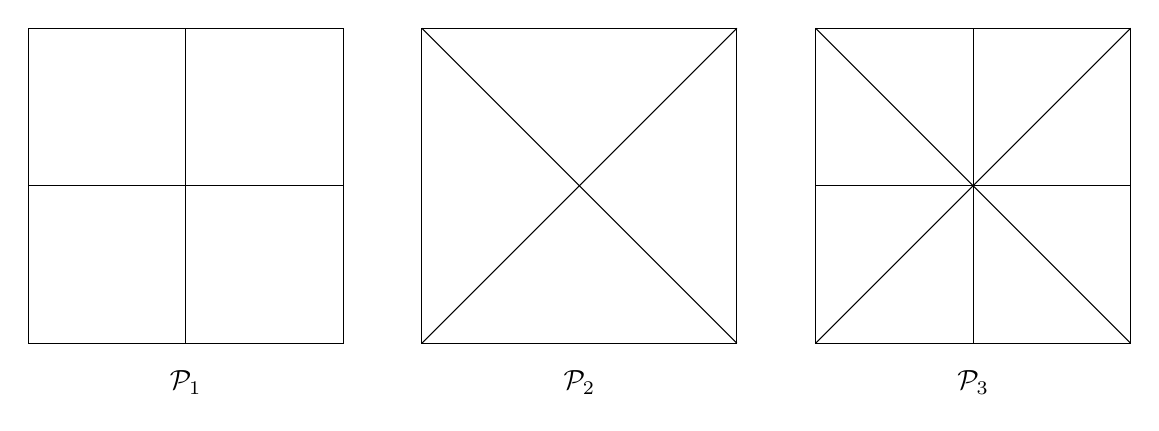
\begin{tikzpicture}
    % Outer square
    \draw (0,0) rectangle (4,4);

    % Vertical and horizontal dividing lines
    \draw (2,0) -- (2,4);
    \draw (0,2) -- (4,2);

    % Outer square
    \draw (5,0) rectangle (9,4);

    % Diagonals
    \draw (5,0) -- (9,4); % Diagonal from bottom-left to top-right
    \draw (5,4) -- (9,0); % Diagonal from top-left to bottom-right
    
    % Outer square
    \draw (10,0) rectangle (14,4);

    % Diagonals
    \draw (10,0) -- (14,4); % Diagonal from bottom-left to top-right
    \draw (10,4) -- (14,0); % Diagonal from top-left to bottom-right
    \draw (10,2) -- (14,2);
    \draw (12,0) -- (12,4);
    
    \node at (2, -0.5) {$\P_1$}; % Label beneath the square
    \node at (7, -0.5) {$\P_2$}; % Label beneath the square
    \node at (12, -0.5) {$\P_3$}; % Label beneath the square
  \end{tikzpicture}
  \caption{Example of 2 partions of the square $\P_1$ and $\P_2$ with common upper bound $\P_3$.}
\end{figure}

\begin{rem}\label{rem:partfinsze}
  If $X$ is an infinite set then $\Pi(X)$ is also infinite.
\end{rem}

\begin{proof}
  Define $\P \subseteq \Pi(X)$ as follows
  \begin{equation*}
    \P := \Big\{ \{ \{x\}, \: X\setminus\{x\}\}\colon \: \forall x \in X \Big\}.
  \end{equation*}
  It is now clear that $\left| \P \right| = \left| X \right|$ and since $\P \subseteq \Pi(X)$ it follows that 
  \begin{equation*}
    \left| X \right| \leq \left| \Pi(X) \right|.
  \end{equation*}
\end{proof}

\clearpage

\topskip0pt
\vspace*{\fill}
\noindent
\textbf{Eidesstattliche Versicherung}

\noindent
Hiermit versichere ich, dass ich die vorliegende Arbeit selbstständig und ohne unerlaubte Hilfe angefertigt und andere als die in der Arbeit angegebenen Hilfsmittel nicht benutzt habe. Alle Stellen, die wörtlich oder sinngemäß aus anderen Schriften entnommen sind, habe ich als solche kenntlich gemacht.
\vspace*{50px}

\noindent
Freiberg, 12. Februar, 2025  
\vspace*{\fill}

\clearpage
\printbibliography

\end{document}
